\documentclass[11pt]{article}
\usepackage[numbers]{natbib}
\usepackage[T1]{fontenc}
\usepackage{bm,amsmath,amsthm,amssymb,multicol,algorithmic,algorithm,enumitem}
\usepackage{wrapfig,lipsum}
\usepackage[textwidth=1cm,textsize=footnotesize]{todonotes}
\usepackage{caption}
% ready for submission
%\usepackage{neurips_2020}
\usepackage[nonatbib,final]{neurips_2020}
\usepackage{thm-restate}
\usepackage{comment}
\usepackage[colorlinks=true,
linkcolor=red,
urlcolor=blue,
citecolor=blue]{hyperref}
\usepackage{hyperref}
\usepackage{cleveref}
\usepackage{subfigure}
\usepackage{booktabs}
\usepackage{mdframed}
\usepackage{thmtools, thm-restate}

\declaretheoremstyle[
    headfont=\bfseries, 
    bodyfont=\normalfont\itshape,
    headpunct={},
    spacebelow=\parsep,
    spaceabove=\parsep,
    mdframed={
        innertopmargin=6pt,
        innerbottommargin=6pt, 
        skipabove=\parsep, 
        skipbelow=\parsep} 
]{framedstyle}

\declaretheorem[
    style=framedstyle,
    name=Theorem
]{thm}

\setlength{\parskip}{.2cm}

 \makeatletter
\renewenvironment{proof}[1][\proofname]{%
   \par\pushQED{\qed}\normalfont%
   \topsep6\p@\@plus6\p@\relax
   \trivlist\item[\hskip\labelsep\bfseries#1]%
   \ignorespaces
}{%
   \popQED\endtrivlist\@endpefalse
}
\makeatother

%%%%%%%%%%% Stuffs for Tikz %%%%%%%%%%%%%%%%%%
\usepackage{pgfplots}
\usepackage{xargs}
\usepackage{stmaryrd}
\usetikzlibrary{arrows,shapes,calc,tikzmark,backgrounds,matrix,decorations.markings}
\usepgfplotslibrary{fillbetween}

\pgfplotsset{compat=1.3}

\usepackage{relsize}
\tikzset{fontscale/.style = {font=\relsize{#1}}
    }

%%%%%%%%%%%%%%%%%%%%%%%%%%%%%%%%%%%%%


\usepackage{shortcuts_OPT}

\makeatletter
\DeclareRobustCommand*\cal{\@fontswitch\relax\mathcal}
\makeatother

\begin{document}
\title{Towards Better Generalization of Adaptive Gradient Methods}

\author{
  Yingxue Zhou, Belhal Karimi, Jinxing Yu, Zhiqiang Xu, Ping Li\\
  Cognitive Computing Lab\\ 
  Baidu Research\\
  No.10 Xibeiwang East Road, Beijing 100193, China\\  
  10900 NE 8th St. Bellevue, Washington 98004, USA\\
  \texttt{\{hustzhouyx,\ belhal.karimi,\ jinxingyu18,\ zhiqiangxu2001,\  pingli98\}@gmail.com}
}

\date{\today}

\maketitle


\begin{abstract}
Adaptive gradient methods such as AdaGrad, RMSprop and Adam have been optimizers of choice for deep learning due to their fast training speed. However, it was recently observed that their generalization performance is often worse than that of SGD for over-parameterized neural networks. While new algorithms such as AdaBound, SWAT, and Padam were proposed to improve the situation, the provided analyses are only committed to optimization bounds for the training objective, leaving critical generalization capacity unexplored. To close this gap, we propose \textit{\textbf{S}table \textbf{A}daptive \textbf{G}radient \textbf{D}escent} (\textsc{SAGD}) for nonconvex optimization which leverages differential privacy to boost the generalization performance of adaptive gradient methods. 
Theoretical analyses show that \textsc{SAGD} has high-probability convergence to a population stationary point. We further conduct experiments on various popular deep learning tasks and models. Experimental results illustrate that \textsc{SAGD} is empirically competitive and often better than baselines. 
\end{abstract}


\section{Introduction}


In this work, we consider the stochastic non-convex optimization~\cite{Proc:Zaheer_NeurIPS18} problem which approximately minimizes the \emph{population loss} given $n $ i.i.d. samples $\z_{1}, \dots, \z_{n}$. Mathematically speaking, we consider the following optimization problem:
\begin{equation} \label{eq: problem}
 \min_{\w \in \cW}~ f({\w})
 \triangleq {\mathbb{E}_{\z \sim \mathcal{P}}}[\ell(\w,\z)]~,
\end{equation}
where $\z\in \mathcal{Z}$ is a data sample in domain $\mathcal{Z}$ following an unknown sample distribution $\mathcal{P}$, ${\w}$ represents the parameter of the underlying learning model, $\ell:\mathcal{W}\times \mathcal{Z}\mapsto \mathbb{R} $ is a certain loss function associated with the learning problem, and the loss function $f$ defined by the population risk is non-convex as with most deep learning tasks. Since  finding the global minimum for non-convex functions
is NP-hard, the utility of a  parameter is usually measured by the $\ell_2$-norm of the gradient. 

Due to the unavailability of distribution $\mathcal{P}$,  the
challenge of a learning algorithm is to search for an approximate minimizer of $f(\w)$ based on only 
$n$ samples $\z_{1}, \dots, \z_{n}$.
A natural approach toward solving the problem stated in \eqref{eq: problem} is empirical risk minimization (ERM)~\citep{Book:Shwartz_2014}, which minimizes the empirical risk:  $\min_{\w \in \cW}  
   \hat f(\w)  \triangleq \frac{1}{n}\sum_{j =1}^{n} \ell(\w, \z_j)~,$
% \begin{equation} \label{eq: empirical}
%   \min_{\w \in \cW}  
%   \hat f(\w)  \triangleq \frac{1}{n}\sum_{j =1}^{n} \ell(\w, \z_j)~,
% \end{equation}
where $\hat f(\w)$ is referred to as empirical risk. 

% We consider in this paper, the following minimization problem:
% \begin{equation} \label{eq: problem}
%  \min_{\w \in \cW}~ f({\w})  \triangleq {\mathbb{E}_{z \sim \mathcal{P}}}[\ell(\w,z)]~,
% \end{equation}
% where the \emph{population loss} $f$ is a (possibly) nonconvex objective function (as for most deep learning tasks), $\cW \subset \R^d$ is the parameter set and $z$ is the vector of data samples distributed according to an unknown data distribution $\mathcal{P}$. 
% We assume that we have access to an oracle that, given $n $ i.i.d. samples $(\z_{1}, \dots, \z_{n})$, returns the stochastic objectives $(\ell(\w,\z_{1}), \dots, \ell(\w,\z_{n}))$.
% Our goal is to find critical points of the population loss function~\eqref{eq: problem}.
% Given the unknown data distribution, a natural approach towards solving \eqref{eq: problem} is empirical risk minimization (ERM)~\citep{Book:Shwartz_2014}, which minimizes the \emph{empirical loss} $\hat f(\w)$ as follows: $\min_{\w \in \cW}     \hat f(\w)  \triangleq \frac{1}{n}\sum_{j =1}^{n} \ell(\w, \z_j)$, when $n$ samples $\z_{1}, \dots, \z_{n}$ are observed.

Stochastic gradient descent (SGD)~\citep{Article:Robbins_1951} which iteratively updates the parameter of a model by descending in the direction of the negative gradient, computed on a single sample or a mini-batch of samples, has been the most dominant algorithm for solving the ERM problem, e.g., training deep neural networks. Since the learning rate has a crucial impact on the convergence and performance of SGD algorithms, there have been studies (e.g.,~\cite{Proc:Chee_AISTATS18}) which automatically tune the
learning rate by reducing it each time a stationarity is detected. A different (and popular) strategy for automatically tuning the learning-rate decay is to use adaptive gradient methods, such as AdaGrad~\citep{Proc:Duchi_JMLR11}, RMSprop~\citep{tige12}, and Adam~\citep{Proc:Kingma_ICLR15}, which have emerged leveraging the curvature of the objective function resulting in adaptive coordinate-wise learning rates for faster convergence.

However, the generalization ability of these adaptive methods is often worse than that of SGD for over-parameterized neural networks, e.g., convolutional neural network (CNN) for image classification and recurrent neural network (RNN) for language modeling~\citep{Proc:Wilson_NIPS17}. 
To mitigate this issue, several recent algorithms were proposed to combine adaptive methods with SGD.
For example, AdaBound~\citep{Proc:Luo_ICLR19} and SWAT~\citep{keso2017} switch from Adam to SGD as the training proceeds, while Padam~\citep{Proc:Chen_IJCAI20, zhta18} unifies AMSGrad~\citep{Proc:Reddi_ICLR18} and SGD with a partially adaptive parameter.  
Despite much efforts on deriving theoretical convergence results of the objective function~\citep{Proc:Zaheer_NeurIPS18,Proc:Ward_ICML19, Proc:Zou_CVPR19, Proc:Chen_ICLR19}, these newly proposed adaptive gradient methods are often misunderstood regarding their generalization abilities, which is the ultimate goal.
On the other hand, current adaptive gradient methods~\citep{Proc:Duchi_JMLR11,Proc:Kingma_ICLR15,tige12, Proc:Reddi_ICLR18, Proc:Ward_ICML19,Proc:Chen_FODS20} follow a typical stochastic optimization (SO) oracle paradigm~\citep{Article:Robbins_1951, Article:Ghadimi_SJO13} which uses stochastic gradients to update the parameters. 
The SO oracle requires \emph{new samples} at every iteration to get the stochastic gradient such that, in expectation, it equals the \emph{population} gradient. 
In practice, however, only finite training samples are available and reused by the optimization oracle for a certain number of times (i.e., epochs). 
~\citep{Proc:Hardt_ICML16} found that the generalization error increases with the number of times the optimization oracle passes over the training data. 
It is thus expected that gradient descent algorithms will be much more well-behaved if we have access to an infinite number of fresh samples. 
Re-using data samples is therefore a caveat for the generalization of a given algorithm.

In order to tackle the above issues, we propose \textit{\textbf{S}table \textbf{A}daptive \textbf{G}radient \textbf{D}escent} (\textsc{SAGD}) which aims at improving the generalization of general adaptive gradient descent algorithms.
\textsc{SAGD} behaves similarly to the aforementioned ideal case of infinite fresh samples borrowing ideas from \emph{adaptive data analysis}~\citep{Proc:Dwork_NIPS15} and \emph{differential privacy}~\citep{Article:Dwork_2014}. 
The main idea of our method is that, at each iteration, \textsc{SAGD} accesses the observations $\z$ through a differentially private mechanism and computes an estimated gradient 
%$\nabla \ell(\w,\z)$ 
of the objective function $\nabla f(\w)$. 
It then uses the estimated gradient to perform a descent step using adaptive stepsize. 
We prove that the reused data points in \textsc{SAGD} nearly possess the statistical nature of \emph{fresh samples} yielding to high concentration bounds of the population gradients through the iterations. \textbf{Our  contributions}  can be summarized as follows:
\begin{itemize}
\item We derive a novel adaptive gradient method, namely \textsc{SAGD}, leveraging ideas of differential privacy and adaptive data analysis aiming at improving the generalization of current baseline methods. A mini-batch variant is also introduced for large-scale learning tasks.
\item Our differentially private mechanism, embedded in the \textsc{SAGD}, explores the idea of Laplace Mechanism (adding Laplace noises to gradients) and \textsc{Thresholdout}~\citep{Article:Dwork_2014} leading to \textsc{DPG-Lap} and \textsc{DPG-Sparse} methods saving privacy cost. 
In particular, we show that differentially private gradients stay close to the population gradients with high probability. 
\item We establish various theoretical guarantees for our algorithm. We derive a concentration bound on the generalization error and show that the $\ell_2$-norm of the \emph{population gradient}, i.e.,  $\|\nabla f(\w)\|$ obtained by the \textsc{SAGD} converges in $\mathcal{O}(1/n^{2/3})$ with high probability. 
\item We conduct several experimental applications based on training neural networks for image classification and language modeling indicating that \textsc{SAGD} outperforms existing adaptive gradient methods in terms of the generalization and over-fitting performance.
\end{itemize}
\textbf{Roadmap:} \ 
The \textsc{SAGD} algorithm, including the differentially private mechanisms, and its mini-batch variant are described in Section~\ref{algorithm}. 
Numerical experiments are presented Section~\ref{sec: experiment}. 
Section~\ref{sec: conclusion} concludes our work. 
Due to space limit, most of the proofs are relegated to supplementary material.

\textbf{Notations:} 
We use $\g_t$ and $\nabla f(\w)$ interchangeably to denote the \emph{population gradient} such that $\g_t = \nabla f(\w_t) = \mathbb{E}_{\z \in \cP} [\nabla \ell(\w_t, \z)]$. 
$S = \left\{\z_{1}, \dots, \z_{n}\right\}$ denotes the $n$ available training samples. 
$\hat \g_t$ denotes the sample gradient evaluated on $S$ such that $\hat \g_t = \nabla \hat f(\w) = \frac{1}{n}\sum_{j=1}^n \nabla \ell(\w_t, \z_j)$. For a vector $\v$, $\v^2$ represents that $\v$ is element-wise squared.  
We use $\v^i$ or $[\v]_i$ to denote the $i$-th coordinate of $\v$ and $\|\v\|_2$ is the $\ell_2$-norm of $\v$ and denote $[d]=\{1,\dots,d\}$.


\section{Preliminaries}


{\bf Adaptive Gradient Methods:} 
In the nonconvex setting, existing work on SGD~\citep{Article:Ghadimi_SJO13} and adaptive gradient methods~\citep{Proc:Zaheer_NeurIPS18, Proc:Ward_ICML19, Proc:Zou_CVPR19, Proc:Chen_ICLR19} show convergence to a stationary point with a rate of  $\mathcal{O}(1/\sqrt{T})$ where $T$ is the number of stochastic gradient computations. Given $n$ samples, a stochastic oracle can obtain at most $n$ stochastic gradients, which implies convergence to the population stationarity with a rate of $\mathcal{O}(1/\sqrt{n})$.
In addition, ~\citep{Proc:Kuzborskij_ICML18, Proc:Raginsky_COLT17, Proc:Hardt_ICML16,Proc:Mou_COLT18, Proc:Pensia_ISIT18, Proc:Chen_ICLR19, Proc:Li_ICLR20} study the generalization of gradient-based optimization algorithms using the generalization property of stable algorithms~\cite{Article:Bousquet_JMLR02}. 
In particular,~\citep{Proc:Raginsky_COLT17, Proc:Mou_COLT18, Proc:Li_ICLR20, Proc:Pensia_ISIT18} focus on noisy gradient algorithms, e.g., \textsc{SGLD}, and provide a generalization error (population risk minus empirical risk) bound in $\mathcal{O}(\sqrt{T}/n)$. 
This type of bounds usually has a dependence on the training data and has a polynomial dependence on $T$.  


\noindent{\bf Differential Privacy and Adaptive Data Analysis:} 
Differential privacy~\cite{Article:Dwork_2014} was originally studied for preserving the privacy of individual data in the statistical query. 
Recently, differential privacy has been widely used for stochastic optimization. 
Some pioneering work~\citep{Article:Chaudhuri_JMLR11, Proc:Bassily_FOCS14,Proc:Wang_NIPS17} introduce differential privacy to empirical risk minimization (ERM) to protect sensitive information of the training data. 
The popular differentially private algorithms include the gradient perturbation that adds noise to the gradient in gradient descent algorithms~\citep{Article:Chaudhuri_JMLR11,Proc:Bassily_FOCS14,Proc:Wang_AAAI19}.
Moreover, in Adaptive Data Analysis \textsc{ADA}~\citep{Proc:Dwork_NIPS15,dwfe2015b,Proc:Dwork_STOC15}, the same holdout set is used multiple times to test the hypotheses which are generated based on previous test results.
It has been shown that reusing the holdout set via a differentially private mechanism ensures the validity of the test. 
In other words, the differentially private reused dataset maintains the statistical nature of fresh samples and improves generalization~\citep{Proc:Zhou_UAI18}. 


\section{Stable Adaptive Gradient Descent Algorithm}\label{algorithm}

Beforehand, we recall the definition of an $(\epsilon, \delta)$-differentially private algorithm:
\begin{defn}
(Differential Privacy~\citep{Article:Dwork_2014}) A randomized algorithm $\mathcal{M}$ is $(\epsilon, \delta)$-differentially private if 
$$\mathbb{P}\{\mathcal{M}(\cal{D})\in \mathcal{Y}\} \leq \exp(\epsilon)\mathbb{P}\{\mathcal{M}(\cal{D\prime})\in \mathcal{Y} \} + \delta$$
holds for all $\mathcal{Y}\subseteq Range(\mathcal{M})$ and all pairs of adjacent datasets $\cal{D},\cal{D\prime}$ that differ on a single sample.
\end{defn}

Intuitively, differential privacy means that the outcomes of two nearly identical datasets should be nearly identical such that an analyst will not be able to distinguish any single data point by monitoring the change of the
output. The general approach for achieving $(\epsilon, \delta)$-differential privacy when estimating a deterministic real-valued function $q: \cZ^n \rightarrow \mathbb{R}^d$ is Laplace Mechanism~\citep{Article:Dwork_2014}, which adds Laplace noise calibrated to the function $q$, i.e.,  $\mathcal{M}(\cD)= q(\cD)+ \b$, where for all $i \in [d]$, $\b^i \sim \textrm{Laplace}(0, \sigma^2)$.
We present \textsc{SAGD} with two different \textbf{D}ifferential \textbf{P}rivate\textbf{ G}radient (DPG) computing methods that provide an estimate of the gradient $\nabla f(\w)$, namely \textsc{DPG-Lap} based on the \emph{Laplace Mechanism}~\citep{Article:Dwork_2014}, see Section~\ref{subsec: SAGD_lap} and an improvement named \textsc{DPG-Sparse} motivated by sparse vector technique~\citep{Article:Dwork_2014} in Section~\ref{subsec: SAGD-sparse}.


\subsection{\textsc{SAGD} with \textsc{DGP-Lap}} \label{subsec: SAGD_lap}


\begin{algorithm}[b] 
\caption{\textsc{SAGD} with \textsc{DGP-Lap}}
\begin{algorithmic}[1] \label{algo: StAda}
\STATE \textbf{Input}: Dataset $S$,  certain loss $\ell(\cdot)$, initial point $\w_0$ and noise level $\sigma$.
\STATE Set  noise level $\sigma$, iteration number $T$,  and stepsize $\eta_t$.
\FOR{$t = 0,...,T-1$}
	\STATE  \textsc{DPG-Lap:} Compute full batch gradient on $S$: \\
	\centerline{ $\hat \g_t = \frac{1}{n} \sum_{j=1}^n\nabla \ell(\w_t, z_j)$.}	
	\STATE \label{line:dpg} Set $\tilde \g_t = \hat \g_t + \b_t$, where $\b_t^i$ is drawn i.i.d from Lap$(\sigma)$ for all $i \in [d]$.
\STATE  \label{line:adap1}
$\m_t = \tilde \g_t$ and $\v_t = \left(1-\beta_{2}\right) \sum_{i=1}^{t} \beta_{2}^{t-i} \tilde \g_{i}^{2}$.
\STATE  \label{line:adap2} $\w_{t+1}=\w_{t}-\eta_t \m_t /(\sqrt{\v_t}+\nu)$.
\ENDFOR 
\end{algorithmic}
\end{algorithm}
In most deep learning applications, a training set $S$ of size $n$ is observed.
Then, at each iteration $t \in [T]$, \textsc{SAGD}, described in Algorithm~\ref{algo: StAda}, calls \textsc{DPG-Lap} (Line~\ref{line:dpg} in Algorithm~\ref{algo: StAda}), that computes the empirical gradient noted $\tilde \g_t$ and updates the model parameter $\w_{t+1}$ using adaptive stepsize.
Note that the noise variance $\sigma^2$, step-size $\eta_t$, iteration number $T$, $~ \beta_2$ are parameters and play an important role for our theoretical study presented in the sequel. 
We first consider \textsc{DPG-Lap} which adds Laplace noise $\b_t \in \mathbb{R}^d$ to the empirical gradient $\hat \g_t = \frac{1}{n} \sum_{j=1}^n\nabla \ell(\w_t, \z_j)$ and returns a noisy gradient $\tilde \g_t = \hat \g_t + \b_t$ to the optimization oracle Algorithm~\ref{algo: StAda}. Throughout the paper, assume:
\begin{assumption}
The objective function $ f: \mathbb{R}^d \rightarrow \mathbb{R}$ is bounded from below by $f^\star$ and is $L$-smooth ($L$-Lipschitz gradients), i.e., $\nr \|\nabla f(\w) -\nabla f(\w^\prime) \|\leq L \|\w-\w^\prime \|$, for all $\w, \w^\prime \in \cW$.
\end{assumption}
\begin{assumption}
The gradient of $\ell$ and its noisy approximation are bounded: For all $\w \in \cW, \  \z \in \cZ$ $\|\nabla \ell (\w, \z) \| \leq G$, for all $t \in [T]$, $\|\tilde \g_t\| \leq G$, and $\|\nabla \ell (\w, z) \|_1 \leq G_1$.
\end{assumption}

To analyze the convergence of SAGD in terms of $\ell_2$ norm of the population gradient, we need to 
show that $\tilde \g_t$ approximate the population gradient $\g_t$ with high probability, i.e., the estimation error $\| \tilde \g_t - \g_t\|$ is small at every iteration.  To make such an analysis, we first present the generalization guarantee of any differentially private algorithm in Lemma~\ref{lem: gen_adv}, and then show that SAGD is differentially private in Lemma~\ref{lemma dpp}. It is followed by establishing SAGD's generalization guarantee in Theorem~\ref{thm: acc_basic}, i.e., estimated $\tilde \g_t$ approximates the population gradient $\g_t$ with high probability.

\textcolor{purple}{\textit{High-probability bound:}} 
We first show that the noisy gradient $\tilde \g_t$ approximates the population gradient $\g_t$ with high probability.
A general approach for analyzing the estimation error
of sample gradient to population gradient is is the Hoeffding's bound, i.e., given training set $S \in \mathcal{Z}^n$, and a fixed $\w_0$ chosen to be independent of the dataset $S$, denote the empirical gradient $\hat \g_0= \mathbb{E}_{z \in S}\nabla \ell(\w_0,z)$ and population gradient $\g_0 = \mathbb{E}_{z\sim \mathcal{P}}[\nabla l(\w_0,z)]$, Hoeffding's bound implies for  $i \in [d]$ and $\mu > 0$:
\begin{equation} \label{hoeffding}
P\{|\hat \g^i_0 - \g_0^i | \geq \mu \} \leq2 \exp \left(\frac{-2n\mu^2}{4G^2} \right)~.
\end{equation}
%   where $G_\infty$ is the maximal value of the $\ell_\infty$-norm of the gradient $ \g_0$. 
Generally, if $\w_1$ is updated using the gradient computed on training set $S$, i.e.,  $\w_1 = \w_0 - \eta \hat \g_0$, concentration inequality~\eqref{hoeffding} \emph{will not} hold for $\hat \g_1 = \mathbb{E}_{z \in S}\nabla_i \ell(\w_1,z)$, because $\w_1$ is no longer independent of $S$. 
However, Lemma~\ref{lem: gen_adv} shows that if $\w_t, \forall\, t \in [T]$ is generated by reusing $S$ under a differentially private mechanism, concentration bounds similar to Eq.~(\ref{hoeffding}) will hold for all $\w_1, \w_2,...,\w_T$ that are adaptively generated on the same dataset $S$. 
% For any differentially private algorithm, Lemma~\ref{lem: gen_adv} provides the following high probability concentration bound:  
\begin{restatable}{lemm}{lemgenadv}
\label{lem: gen_adv}
	Let $\cA$ be an $(\epsilon, \delta)$-differentially private gradient descent algorithm with access to training set $S$ of size $n$. Let $\w_t = \cA(S)$ be the parameter generated at iteration $t \in [T]$ and $\hat \g_t$ the empirical gradient on $S$. For any $\sigma >0$, $\beta > 0$, if the privacy cost of $\cA$ satisfies $\epsilon \leq \sigma/13$, $\delta \leq \sigma \beta/(26 \ln(26/\sigma))$, and sample size $n \geq 2\ln(8/\delta)/\epsilon^2$, we then have
	\begin{equation*}
	\mathbb{P}\left\{ |\hat \g_t^i - \g_t^i| \geq  G \sigma \right\} \leq \beta~, \quad \textrm{$ \forall i\in [d]$ and  $\forall t \in [T]$} ~.
	\end{equation*} 
\end{restatable}
Lemma~\ref{lem: gen_adv} is an instance of Theorem 8 from~\cite{Proc:Dwork_NIPS15} and illustrates that, if the privacy cost $\epsilon$ is bounded by the estimation error, the differential privacy mechanism enables the reused training samples set to maintain statistical guarantees as if they were fresh samples. 
Then, we establish in Lemma~\ref{lemma dpp}, that \textsc{SAGD} with \textsc{DPG-Lap} is a differentially private algorithm with the following privacy cost:
\begin{restatable}{lemm}{lemdpp}
\label{lemma dpp}
\textsc{SAGD} with \textsc{DPG-Lap} (Alg.~\ref{algo: StAda}) is $(\frac{\sqrt{T \ln(1/\delta)} G_1}{n\sigma}, \delta)$-differentially private. 
\end{restatable}  
In order to achieve a gradient concentration bound for \textsc{SAGD} with \textsc{DPG-Lap} as described in Lemma~\ref{lem: gen_adv}, we set $\sqrt{T \ln(1/\delta)} G_1/(n\sigma)\leq \sigma/13$, $\delta \leq \sigma \beta/(26 \ln(26/\sigma))$, and  sample size $n \geq 2\ln(8/\delta)/\epsilon^2$. 
Then, the following result shows that across all iterations, gradients produced by \textsc{SAGD} with \textsc{DPG-Lap} maintain high probability concentration bounds.\\

\begin{restatable}{thm}{theoaccbasic}
\label{thm: acc_basic}
Given $\sigma > 0$, let $\tilde \g_1,...,  \tilde \g_T$ be gradients computed by \textsc{DPG-Lap} in \textsc{SAGD}. Set the number of iterations $ 2n\sigma^2/G_1^2\leq T \leq n^2 \sigma^4/(169 \ln(1/(\sigma \beta))G_1^2)$, then for $t \in [T]$, $\beta >0$, $\mu > 0$:
    \begin{equation*}
    \mathbb{P}\left\{\|\tilde \g_t - \g_t\| \geq \sqrt{d}\sigma(G +\mu)\right\} \leq d\beta + d\exp(-\mu)~.
    \end{equation*}
\end{restatable}
Note that given the concentration error bound of $\sqrt{d}\sigma(G +\mu)$, Theorem~\ref{thm: acc_basic} indicates that a higher noise level $\sigma$, implying a better privacy guarantee and a larger number of iterations $T$,would meanwhile incur a larger concentration error.
Thus, there is a trade-off between noise and accuracy illustrated by the positive numbers $\beta$ and $\mu$.
A larger $\mu$ brings a larger concentration error but a smaller probability. 
A larger $\beta$ implies a larger upper bound on $T$, yet also a larger probability bound. We
optimize the choice of $\beta$ and $\mu$ for analyzing the
convergence to the population stationary point.
%Note that although the probability $d\beta + d\exp(-\mu)$ has a dependence on dimension $d$, we can choose appropriate $\beta$ and $\mu$ to make the probability arbitrarily small when analyzing the convergence to a stationary point.

\textcolor{purple}{\textit{Non-asymptotic convergence rate:}}
We derive the optimal values of $\sigma$ and $T$ to improve the trade-off between the statistical rate and the optimization rate and we obtain a novel finite-time bound in Theorem~\ref{thm: main_rmsprop}. 
Denote $\rho_{n,d} \triangleq\mathcal{O} \left(\ln n + \ln d\right)$, we prove that \textsc{SAGD} with \textsc{DPG-Lap} converges to a population stationary point with high probability at the following rate:

\vspace{0.08in}

\begin{restatable}{thm}{theomainrmsprop}
\label{thm: main_rmsprop}
 Given training set $S$ of size $n$, for $\nu >0$, if $\eta_t = \eta$  with $\eta \leq \nu/(2L)$,  $\sigma = 1/n^{1/3}$, iteration number $T = n^{2/3}/\left(169G_1^2(\ln d +7\ln n/3)\right)$, $\mu = \ln (1/\beta)$ and $\beta = 1/(d n^{5/3})$, then \textsc{SAGD} with \textsc{DPG-Lap} algorithm yields:
 \begin{small}
\begin{equation*}
 \min_{1\leq t \leq T}\|\nabla f(\w_t)\|^2 \leq
\mathcal{O} \left( \frac{\rho_{n,d} \left(f(\w_1) - f^\star \right)}{n^{2/3}} \right) + \mathcal{O} \left( \frac{d \rho_{n,d}^2}{n^{2/3}}\right)~,
\end{equation*}
\end{small}
with probability at least $1-\mathcal{O} \left(1/(\rho_{n,d} n)\right)$.
\end{restatable} 
Theorem~\ref{thm: main_rmsprop} shows that, given $n$ samples, \textsc{SAGD} converges to a stationary point at a rate of $\mathcal{O}(1/n^{2/3})$ where we use the $\ell_2$ norm of the gradient of the objective function as a convergence criterion.
Particularly, the first term of the bound corresponds to the optimization error $\mathcal{O}(1/T)$ with $T = \mathcal{O}(n^{2/3})$, while the second is the statistical error depending on available sample size $n$ and dimension $d$. 
%In terms of computation complexity, \textsc{SAGD} requires $\mathcal{O}(n^{5/2})$ stochastic gradient computations for $\mathcal{O}(n^{3/2})$ passes over $n$ samples. 
The current optimization analyses~\citep{Proc:Zaheer_NeurIPS18, Proc:Ward_ICML19, Proc:Zou_CVPR19, Proc:Chen_ICLR19} show that adaptive gradient descent algorithms converge to the stationary point of the objective function with a rate of $\mathcal{O}(1/\sqrt{T})$ with $T$ stochastic gradient computations. 
Given $n$ samples, their analyses yield a rate of  $\mathcal{O}(1/\sqrt{n})$. 
Thus, the \textsc{SAGD} achieves a sharper bound compared to the previous analyses. 

\subsection{\textsc{SAGD} with \textsc{DPG-Sparse}} \label{subsec: SAGD-sparse}


In this section, we consider the \textsc{SAGD} with an advanced version of \textsc{DPG} named \textsc{DPG-Sparse} motivated by the sparse vector technique~\citep{Article:Dwork_2014} aiming to provide a sharper result on the privacy cost $\epsilon$ and $\delta$.
Lemma~\ref{lemma dpp} shows that the privacy cost of \textsc{SAGD} with \textsc{DPG-Lap} scales with $\mathcal{O}(\sqrt{T})$. In order to guarantee the generalization of \textsc{SAGD} as stated in Theorem~\ref{thm: acc_basic}, we need to control the privacy cost below a certain threshold i.e.,  $\sqrt{T \ln(1/\delta)} G_1/(n\sigma) \leq \sigma/13$. However, it limits the iteration number $T$ of \textsc{SAGD}, leading to a compromised optimization term in Theorem~\ref{thm: main_rmsprop}.  
In order to relax the upper bound on $T$, we propose the \textsc{SAGD} with \textsc{DPG-Sparse} in Algorithm~\ref{algo: sparse}.
Given $n$ samples, Algorithm~\ref{algo: sparse} splits the dataset evenly into two parts $S_1$ and $S_2$. 
At each iteration $t$, Algorithm~\ref{algo: sparse} computes gradients on both datasets:
$\hat \g_{S_1,t} = \frac{1}{|S_1|} \sum_{\z_j \in S_1}\nabla \ell(\w_t, \z_j)$ and $\hat \g_{S_2,t} = \frac{1}{|S_2|} \sum_{\z_j \in S_2}\nabla \ell(\w_t, \z_j)$.
It then validates $\hat \g_{S_1,t} $ with $\hat \g_{S_2,t}$, i.e., \ if the norm of their difference is greater than a random threshold $\tau-\gamma$, it returns $\tilde \g_t = \hat \g_{S_1,t} + \b_t$, otherwise $\tilde \g_t = \hat \g_{S_2,t}$.

\begin{algorithm}[H]
\caption{\textsc{SAGD} with \textsc{DPG-Sparse}}
\begin{algorithmic}[1]
\label{algo: sparse}
\STATE \textbf{Input}: Dataset $S$,  certain loss $\ell(\cdot)$, initial point $\w_0$.
%sequence of functions $\{\phi_t, \psi_t \}_{t=0}^{T-1}$
\STATE Set  noise level $\sigma$, iteration number $T$,  and stepsize $\eta_t$.
\STATE Split $S$ randomly into $S_1$ and $S_2$. 
\FOR{$t = 0,...,T-1$}
\STATE   \textsc{DPG-Sparse:} Compute full batch gradient on $S_1$ and $S_2$:\\
\centerline{$\hat \g_{S_1,t} = \frac{1}{|S_1|} \sum_{\z_j \in S_1}\nabla \ell(\w_t, \z_j)$,%}
%\centerline{
\hspace{0.2in}
$\hat \g_{S_2,t} = \frac{1}{|S_2|} \sum_{\z_j \in S_2}\nabla \ell(\w_t, \z_j)$.}
\STATE Sample $\gamma \sim \text{Lap}(2\sigma)$, $\tau \sim \text{Lap}(4\sigma)$.
\IF{$\| \hat \g_{S_1,t} - \hat \g_{S_2,t}\| + \gamma >  \tau$}
\STATE  $\tilde \g_t = \hat \g_{S_1,t} + \b_t$, where $\b_t^i$ is drawn i.i.d from Lap$(\sigma)$, for all $ i \in [d]$.
\ELSE \STATE $\tilde \g_t = \hat \g_{S_2,t}$
\ENDIF
\STATE 
$\m_t = \tilde \g_t$ and $\v_t = \left(1-\beta_{2}\right) \sum_{i=1}^{t} \beta_{2}^{t-i} \tilde \g_{i}^{2}$.
%$\m_t = \phi_t(\tilde \g_1, ..., \tilde \g_t)$ and $\v_t = \psi_t(\tilde \g_1,.., \tilde \g_t)$
\STATE $\w_{t+1}=\w_{t}-\eta_t \m_t /(\sqrt{\v_t}+\nu)$.
\ENDFOR 
\STATE \textbf{Return}: $\tilde \g_t$.
\end{algorithmic}
\end{algorithm}

Following \textsc{Thresholdout},~\citep{Proc:Zhou_UAI18} propose a stable gradient descent algorithm which uses a similar framework as \textsc{DPG-Sparse} to compute an estimated gradient by validating each coordinate of $\hat \g_{S_1,t}$ and $\hat \g_{S_2,t}$. 
Thus, their method is computationally expensive in high-dimensional settings such as deep neural networks. 
%Ours are particularly suited for those models, as observed in Section~\ref{sec: experiment}.

\textcolor{purple}{\textit{High-probability bound:}}
To analyze the privacy cost of \textsc{DPG-Sparse}, let $C_{s}$ be the number of times the validation fails, i.e.,  $\| \hat \g_{S_1,t} - \hat \g_{S_2,t}\| + \gamma >  \tau$ is true, over $T$ iterations in \textsc{SAGD}. The following Lemma establishes the privacy cost of the \textsc{SAGD} with \textsc{DPG-Sparse} algorithm.
\begin{restatable}{lemm}{lemdppsparse}
\label{lemma: dpp-sparse}
\textsc{SAGD} with \textsc{DPG-Sparse}  (Alg.~\ref{algo: sparse}) is  
$(\frac{\sqrt{C_{s} \ln(2/\delta)} 2G_1}{n\sigma}, \delta)$-differentially private. 
\end{restatable}
Lemma~\ref{lemma: dpp-sparse} shows that the privacy cost of  \textsc{SAGD} with \textsc{DPG-Sparse} scales with $\mathcal{O}(\sqrt{C_{s}})$ where $C_{s} \leq T$. 
In other words, \textsc{DPG-Sparse} procedure improves the privacy cost of the \textsc{SAGD} algorithm. 
Indeed, in order to achieve the generalization guarantee of \textsc{SAGD} with \textsc{DPG-Sparse}, stated in Lemma~\ref{lem: gen_adv} and  by considering the result of Lemma~\ref{lemma: dpp-sparse},  we only need to set $\sqrt{C_{s} \ln(1/\delta)} G_1/(n\sigma) \leq \sigma/13$, which potentially improves the upper bound on $T$. 
We derive the generalization guarantee of $\tilde \g_t$ generated by the \textsc{SAGD} with \textsc{DPG-Sparse} algorithm in the following result:

\vspace{0.1in}

\begin{restatable}{thm}{theoaccsparse}
\label{thm: acc_sparse}
Given $\sigma > 0$, let $\tilde \g_1,...,  \tilde \g_T$ be the gradients computed by \textsc{DPG-Sparse} in \textsc{SAGD}. With a budget $ n\sigma^2/(2G_1^2) \leq C_{s} \leq n^2 \sigma^4/(676 \ln(1/(\sigma \beta))G_1^2)$, then for $t \in [T]$,$\beta > 0$, $\mu > 0$:
        \begin{equation*}
    \mathbb{P}\left\{\|\tilde \g_t - \g_t\| \geq \sqrt{d}\sigma(1+\mu)\right\} \leq d\beta + d\exp(-\mu)~.
    \end{equation*}
\end{restatable}
In the worst case $C_{s} = T$, we recover the bound of $T \leq n^2 \sigma^4/(676 \ln(1/(\sigma \beta))G_1^2)$ of \textsc{DPG-Lap}.

\textcolor{purple}{\textit{Non-asymptotic convergence rate:}}
The finite-time upper bound on the convergence criterion of interest for the \textsc{SAGD} with \textsc{DPG-Sparse} algorithm (Algorithm~\ref{algo: sparse}) is stated as follows:

\vspace{0.1in}

\begin{restatable}{thm}{theormspropsparse}
\label{thm: main_rmsprop_sparse}
 Given training set $S$ of size $n$, for $\nu >0$, if $\eta_t = \eta$ which are chosen with $\eta \leq \nu/(2L)$, noise level $\sigma = 1/n^{1/3}$, and iteration number $T = n^{2/3}/\left(676G_1^2(\ln d + \frac{7}{3}\ln n)\right)$, then \textsc{SAGD} with \textsc{DPG-Sparse} algorithm yields:
  \begin{small}
\begin{equation*}
 \min_{1\leq t\leq T}\|\nabla f(\w_t)\|^2 \leq
\mathcal{O} \left( \frac{\rho_{n,d} \left(f(\w_1) - f^\star \right)}{n^{2/3}} \right) +\mathcal{O} \left( \frac{d \rho_{n,d}^2}{n^{2/3}}\right)~,
\end{equation*}
\end{small}
with probability at least $1-\mathcal{O} \left(1/(\rho_{n,d} n)\right)$.
\end{restatable} 
Theorem~\ref{thm: main_rmsprop_sparse} displays a similar rate of $\mathcal{O}(1/n^{2/3})$ for the \textsc{SAGD} with \textsc{DGP-Sparse} as Theorem~\ref{thm: main_rmsprop}. 
A sharper bound can be achieved when the number of validation failures $C_{s}$ is smaller than $T$. 
For example, if $C_{s} = \mathcal{O}(\sqrt{T})$, the upper bound of $T$ can be improved from $T \leq \mathcal{O}(n^2)$ to $T \leq \mathcal{O}(n^4)$.



\subsection{Mini-batch Stable Adaptive Gradient Descent Algorithm}
\label{mini-batch algorithm}


For large-scale learning we derive the mini-batch variant of \textsc{SAGD} in Algorithm~\ref{algo: mini-StAda}. 
The training set $S$ is first partitioned into $B$ batches with $m$ samples for each batch. 
At each iteration $t$, Algorithm~\ref{algo: mini-StAda} uses any \textsc{DPG} procedure to compute a differential private gradient $\tilde \g_t$ on each batch and updates $\w_t$. 
\begin{algorithm}[H]
\caption{Mini-Batch \textsc{SAGD}}
\begin{algorithmic}[1] \label{algo: mini-StAda}
\STATE \textbf{Input}: Dataset $S$,  certain loss $\ell(\cdot)$, initial point $\w_0$.
%, initialize $t=0$
%, sequence of functions $\{\phi_t, \psi_t \}_{t=1}^T$
\STATE Set noise level $\sigma$, epoch number $T$,  batch size $m$, and stepsize $\eta_t$.
\STATE Split $S$ into $B=n/m$ batches: $\{ s_1,..., s_B\}$.
\FOR{$epoch = 1,...,T$}
\FOR{$k = 1,..., B$}
\STATE \label{line:dpgmini} Call \textsc{DPG-Lap} or \textsc{DPG-Sparse} to compute $\tilde \g_t$.
\STATE \label{line:mini1} $\m_t = \tilde \g_t$ and $\v_t = \left(1-\beta_{2}\right) \sum_{i=1}^{t} \beta_{2}^{t-i} \tilde \g_{i}^{2}$.
%$\m_t = \phi_t(\tilde \g_1, ..., \tilde \g_t)$ and $\v_t = \psi_t(\tilde \g_1,.., \tilde \g_t)$
\STATE \label{line:mini2} $\w_{t+1}=\w_{t}-\eta_t \m_t /(\sqrt{\v_t}+\nu)$.
\ENDFOR
\ENDFOR 
\end{algorithmic}
\end{algorithm} 

Theorem~\ref{thm: main_rmsprop_mini} 
describes the convergence rate of the mini-batch \textsc{SAGD} algorithm in terms of batch size $m$ and sample size $n$, i.e.,  $\mathcal{O}(1/(mn)^{1/3})$.

\vspace{0.1in}

\begin{restatable}{thm}{theomini}
\label{thm: main_rmsprop_mini}
Consider the mini-batch \textsc{SAGD} with \textsc{DPG-Lap}. 
Given $S$ of size $n$, with $\nu >0$, $\eta_t = \eta \leq \nu/(2L)$, noise level $\sigma = 1/(mn)^{1/6}$, and epoch $T = m^{4/3}/\left(n^{2/3}169G_1^2(\ln d + \frac{7}{3}\ln n)\right)$, then:
 \begin{small}
\begin{equation*}
\begin{split}
 \min_{t = 1,..., T}\|\nabla f(\w_t)\|^2 
 \leq\mathcal{O} \left( \frac{\rho_{n,d} \left(f(\w_1) - f^\star \right)}{(mn)^{1/3}} \right)+\mathcal{O} \left( \frac{d \rho_{n,d}^2}{(mn)^{1/3}}\right)~,
 \end{split}
\end{equation*}
\end{small}
with probability at least $1-\mathcal{O} \left(1/(\rho_{n,d} n)\right)$.
\end{restatable}
When $m = \sqrt{n}$, mini-batch \textsc{SAGD} achieves the convergence of rate $\mathcal{O}(1/\sqrt{n})$. When $m=n$, i.e.,  in the full batch setting, Theorem~\ref{thm: main_rmsprop_mini} recovers \textsc{SAGD}'s convergence rate  $\mathcal{O}(1/n^{2/3})$. 
In terms of computational complexity, the mini-batch \textsc{SAGD} requires $\mathcal{O}(m^{4/3}n^{1/3})$ stochastic gradient computations for $\mathcal{O}(m^{4/3}/n^{2/3})$ passes over $n$ samples, while \textsc{SAGD} requires $\mathcal{O}(n^{5/3})$ stochastic gradient computations. 
Thus, the mini-batch \textsc{SAGD} has the advantage of decreasing the computation complexity, but displays a slower convergence than \textsc{SAGD}.





\section{Numerical Experiments} \label{sec: experiment}


In this section, we evaluate our proposed mini-batch \textsc{SAGD} algorithm on various deep learning models against popular optimization methods: SGD with momentum~\citep{Article:Qian_NN99}, Adam~\citep{Proc:Kingma_ICLR15},  RMSprop~\citep{tige12}, and Adabound~\citep{Proc:Luo_ICLR19}. 
We consider three tasks: the classification tasks on MNIST~\citep{Article:Lecun_IEEE98} and CIFAR-10~\citep{krhi2009}, and the language modeling task on Penn Treebank~\citep{Article:Marcus_CL93} and the SNLI dataset~\citep{Proc:Bowman_EMNLP15}, corpus of $570 \, 000$ human-written English sentence pairs where the goal is to predict if an hypothesis is an \emph{entailment}, \emph{contradiction} or \emph{neutral} with respect to a given text.

The setup of each task is given in the following table:
 \begin{table}[H]
 	\centering
 	\label{tab::network_setup}
	\resizebox{\columnwidth}{!}{%
 	\begin{tabular}{lll}	
 	\toprule%[2pt]
 	\textbf{Dataset} & \textbf{Network Type}    & \textbf{Architectures} \\ 	
 	\midrule%[1pt]
 		MNIST            & Feedforward     & 2-Layer with ReLU  and 2-Layer with Sigmoid  \\
 		CIFAR-10         & Deep Convolutional       & VGG-19 and ResNet-18                \\
 		Penn Treebank    & Recurrent                & 2-Layer LSTM and 3-Layer LSTM      \\
 		SNLI    & Recurrent                & bidirectional LSTM      \\
 		\bottomrule%[1pt]
 	\end{tabular}
	}
 \end{table}


\subsection{Environmental Settings}


\textbf{Datasets and Evaluation Metrics:}  The MNIST dataset has a training set of 60000 examples and a test set of 10000 examples. The CIFAR-10 dataset consists of 50000 
training images and 10000 test images. The Penn Treebank dataset contains 929589, 73760, and 82430 tokens for training, validation, and test,  respectively.
To better understand the generalization ability of each optimization algorithm with an increasing training sample size $n$, for each task, we construct multiple training sets of different size by sampling from the original training set. For MNIST, training sets of size $n \in \{50, 100, 200, 500, 10^3, 2.10^3, 5.10^3, 10^4, 2.10^4, 5.10^4 \}$ are constructed. For CIFAR10, training sets of size $n \in \{ 200, 500, 10^3, 2.10^3, 5.10^3, 10^4, 2.10^4,3.10^4, 5.10^4\}$ are constructed. 
For each $n$, we train the model and report the loss and accuracy on the test set.  
For Penn Treebank and SNLI, all training samples are used to train the model and we report the training perplexity and the test perplexity across~epochs. 
%We choose the settings achieving the lowest final training loss.
Cross-entropy is used as the loss function throughout experiments. The mini-batch size is set to be 128 for CIFAR10 and MNIST, 20 for Penn Treebank and SNLI. 
We repeat each experiment 5 times and report the mean of the results.

\vspace{0.05in}

\textbf{Hyper-parameter setting:} 
Optimization hyper-parameters affect the quality of solutions. 
Particularly,~\citep{Proc:Wilson_NIPS17} highlight that the initial stepsize and the scheme of decaying stepsizes have a considerable impact on the performance. 
We follow the logarithmically-spaced grid method in~\citep{Proc:Wilson_NIPS17} to tune the stepsize. 
%Specifically, we start with a logarithmically-spaced grid of four stepsizes. 
If the parameter performs best at an extreme end of the grid, a new grid will be tried until the best parameter lies in the middle of the grid. 
Once the interval of the best stepsize is located, we change to the linear-spaced grid to further search for the optimal one. 
We specify the strategy of decaying stepsizes in the subsections of each task. 
For each experiment, we set $\sigma^2 = 1/n^{2/3}$, where $n$ is the size of the training set, as stated in Theorem~\ref{thm: main_rmsprop_mini}. 
Parameters $\nu$, $\beta_2$, and $T$ follow the default settings as adaptive algorithms such as RMSprop. 

\subsection{Numerical results}\label{subsec:results}


\begin{figure}[t]
\mbox{
\includegraphics[width=1.45in]{fig2/MNIST_ReLU_loss.eps}
\hspace{-0.15in}
\includegraphics[width=1.45in]{fig2/MNIST_ReLU_acc.eps}
\hspace{-0.15in}
\includegraphics[width=1.45in]{fig2/MNIST_Sigmoid_loss.eps}
\hspace{-0.15in}
\includegraphics[width=1.45in]{fig2/MNIST_Sigmoid_acc.eps}
}
 \mbox{
\includegraphics[width=1.45in]{fig2/CIFAR_Resnet_loss.eps}
\hspace{-0.15in}
\includegraphics[width=1.45in]{fig2/CIFAR_Resnet_acc.eps}
\hspace{-0.15in}
\includegraphics[width=1.45in]{fig2/CIFAR_VGG_loss.eps}
\hspace{-0.15in}
\includegraphics[width=1.45in]{fig2/CIFAR_VGG_acc.eps}
}
 \caption{ Test loss and accuracy of ReLU neural network and Sigmoid neural network on MNIST. In both cases, \textsc{SAGD} obtains the best test accuracy among all the methods. Test loss and accuracy of ResNet-18 andVGG-19 on CIFAR10. \textsc{SAGD} achieves the lowest test loss. For VGG-19, \textsc{SAGD} achieves the best test accuracy among all the methods. 
The x-axis is the number of train samples, and the y-axis is the testing loss/accuracy.} 
 \label{fig:mnist}
\end{figure}

% \begin{figure}[t]
% \mbox{
% \subfigure[MNIST, 2-layer ReLU]{
% \hspace{-0.15in}
% 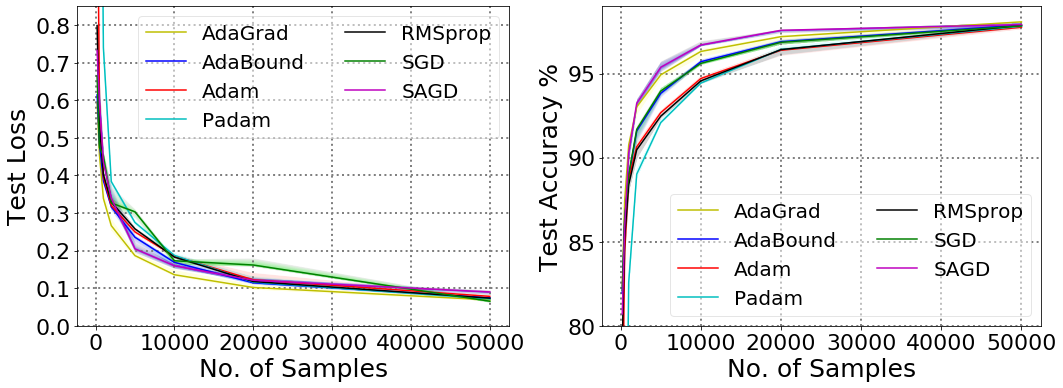
\includegraphics[width = 0.50 \textwidth]{figure/new/relu_lap.png}
% }
% \hspace{-0.1in}
% \subfigure[MNIST, 2-layer Sigmoid]{
% 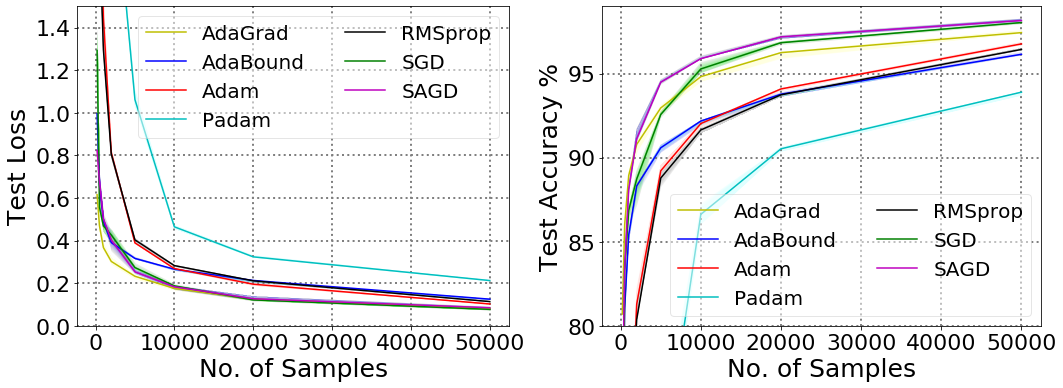
\includegraphics[width = 0.50 \textwidth]{figure/new/sigmoid_lap.png}
%  }
%  }


%  \mbox{
% \subfigure[CIFAR10, ResNet-18]{
% \hspace{-0.15in}
% 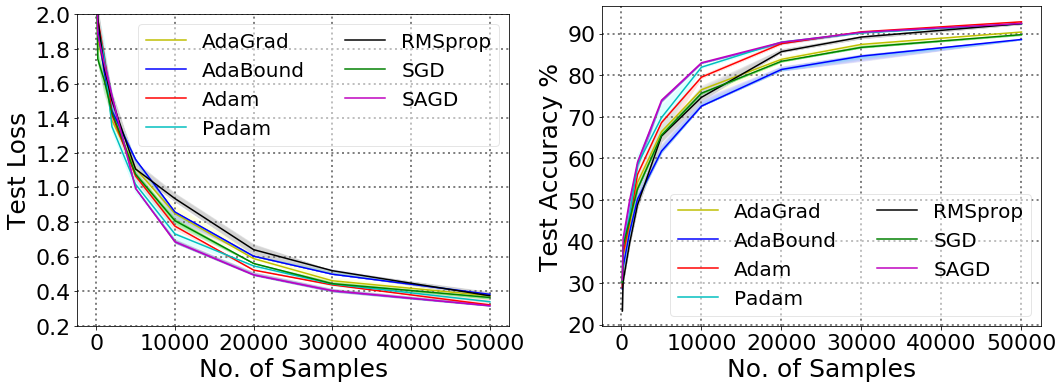
\includegraphics[width = 0.50 \textwidth]{figure/new/resnet200ep.png}
% }
% \hspace{-0.1in}
% \subfigure[CIFAR10, VGG-19]{
% 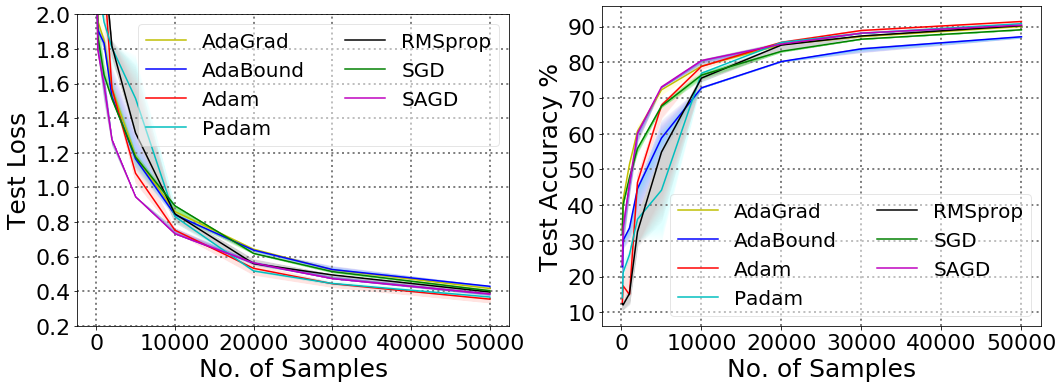
\includegraphics[width = 0.50 \textwidth]{figure/new/vgg200ep.png}
%  }
%  }
%  \caption[]{ \textbf{Top row}: Test loss and accuracy of (a) ReLU neural network and (b) Sigmoid neural network on MNIST. The X-axis is the number of train samples, and the Y-axis is the loss/accuracy. In both cases, \textsc{SAGD} obtains the best test accuracy among all the methods.
% \textbf{Bottom row}: Test loss and accuracy of ResNet-18 andVGG-19 on CIFAR10. \textsc{SAGD} achieves the lowest test loss. For VGG-19, \textsc{SAGD} achieves the best test accuracy among all the methods. } 
%  \label{fig:mnist}
% \end{figure}

%\vspace{0.05in}

\textbf{Feedforward Neural Network.}
For image classification on MNIST, we focus on two 2-layer fully connected neural networks with either ReLU or Sigmoid activation functions. 
We run 100 epochs and decay the learning rate by 0.5 every 30 epochs. 
Figure~\ref{fig:mnist} presents the loss and accuracy on the test set given different training set sizes. 
Since all algorithms attain the $100\%$ training accuracy, the performance on the training set is omitted. 
Figure~\ref{fig:mnist} shows that, for ReLU neural network, \textsc{SAGD} performs slightly better than the other algorithms in terms of test accuracy. When $n =50000$, \textsc{SAGD} gets a test accuracy of $98.98 \pm 0.01 \%$. 
Figure~\ref{fig:mnist} also presents the results on Sigmoid neural network where \textsc{SAGD} achieves the best test accuracy among all the algorithms. When $n =50000$, \textsc{SAGD} reaches the highest test accuracy of $98.04 \pm 0.02 \%$, outperforming other adaptive algorithms.

\vspace{0.05in}

\textbf{Convolutional Neural Network.}
We use ResNet-18~\citep{Proc:He_CVPR16} and VGG-19~\citep{Proc:Simonyan_ICLR15} for the CIFAR-10 image classification task. 
We run 200 epochs and decay the learning rate by 0.1 every 30 epochs. 
% The results are presented in Figure~\ref{fig:mnist}. 
Figure~\ref{fig:mnist} shows that \textsc{SAGD} has higher test accuracy than the 
other algorithms when the sample size is small i.e.,  $n \leq 20000$.
When $n = 50000$, \textsc{SAGD} achieves nearly the same test accuracy, $92.44 \pm 0.07\%$,  as Adam and RMSprop on ResNet-18.
Non-adaptive algorithm SGD performs better than the other algorithms in terms of test loss. 
%Regarding the test accuracy, the \textsc{SAGD}, Adam Padam, and SGD perform better than the other.
Figure~\ref{fig:mnist} also reports the results on VGG-19. Although \textsc{SAGD} has a higher test loss than the other algorithms, it achieves the best test accuracy, especially when $n$ is small. 
Adam and our method performs better than the other adaptive gradient algorithms regarding the test accuracy.
When $n= 50000$, Adam has the best test accuracy $91.42 \pm 0.04\%$. \textsc{SAGD} achieves accuracy $91.26 \pm 0.05\%$.


\begin{figure}[t]
\mbox{
\includegraphics[width=1.86in]{fig2/PTB_2LSTM_train.eps}
\hspace{-0.12in}
\includegraphics[width=1.86in]{fig2/PTB_3LSTM_train.eps}
\hspace{-0.12in}
\includegraphics[width=1.86in]{fig2/SNLI_biLSTM_train.eps}
}
\mbox{
\includegraphics[width=1.86in]{fig2/PTB_2LSTM_test.eps}
\hspace{-0.12in}
\includegraphics[width=1.86in]{fig2/PTB_3LSTM_test.eps}
\hspace{-0.12in}
\includegraphics[width=1.86in]{fig2/SNLI_biLSTM_test.eps}
}
\vspace{-0.1in}
  \caption{Train and test perplexity of 2-layer LSTM (2LSTM),  3-layer LSTM (3LSTM) and biLSTM. 
 Although some baseline optimizers achieve better training performance than \textsc{SAGD}, the latter performs the best in terms of the test perplexity among all the methods.
} 
 \label{fig:language}\vspace{-0.05in}
\end{figure}


%\begin{figure}[t] 
% \mbox{
%\subfigure[Penn Treebank, 2-Layer LSTM]{
%%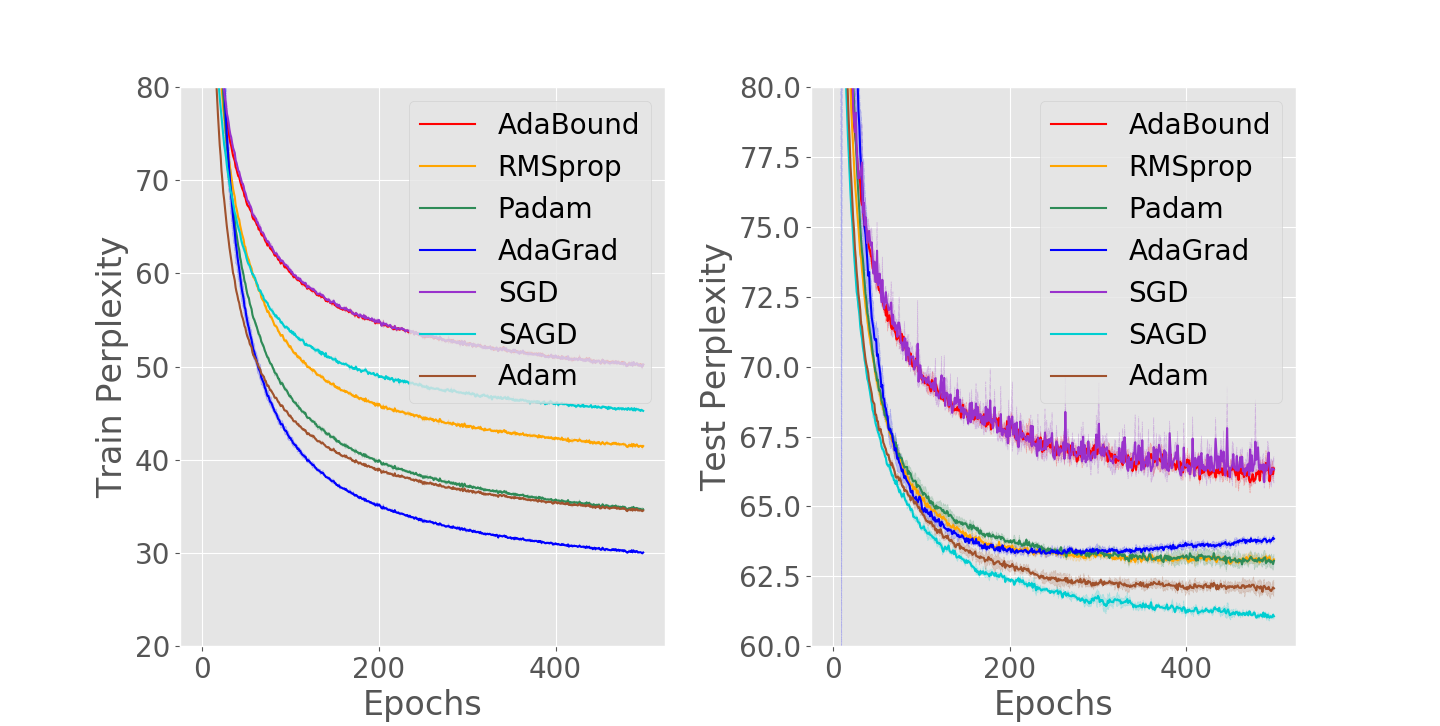
\includegraphics[width = 0.52 \textwidth]{figure/ptb_2lstm.png}
%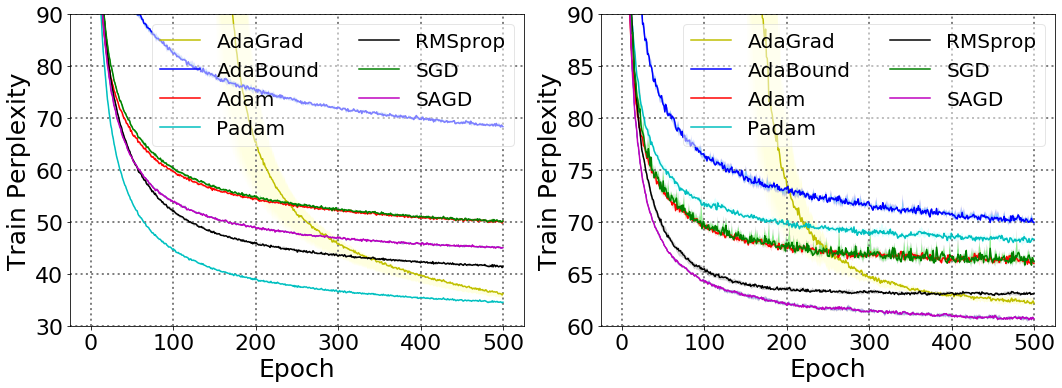
\includegraphics[width = 0.48 \textwidth ]{figure/new/2lstm_lap.png}
%}
%\subfigure[Penn Treebank, 3-Layer LSTM]{
%%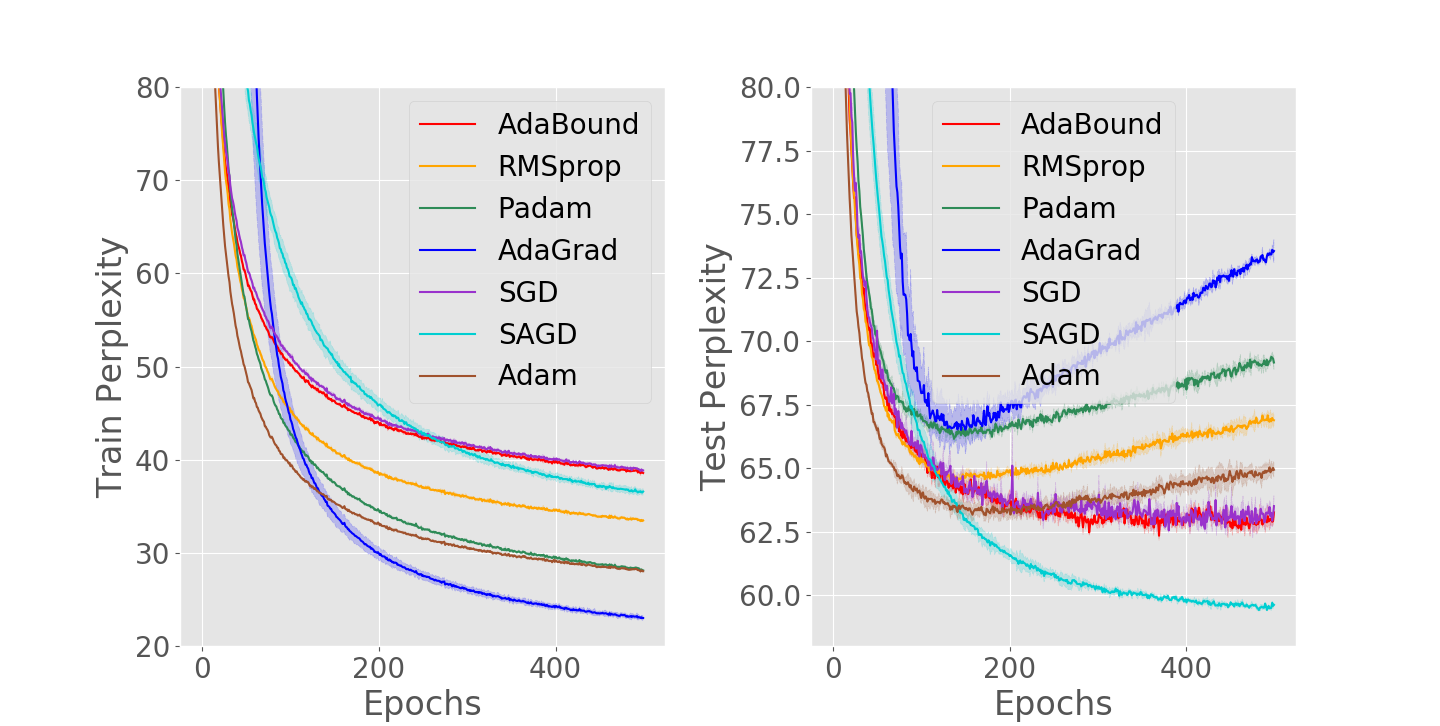
\includegraphics[width = 0.52 \textwidth]{figure/ptb_3lstm.png}
%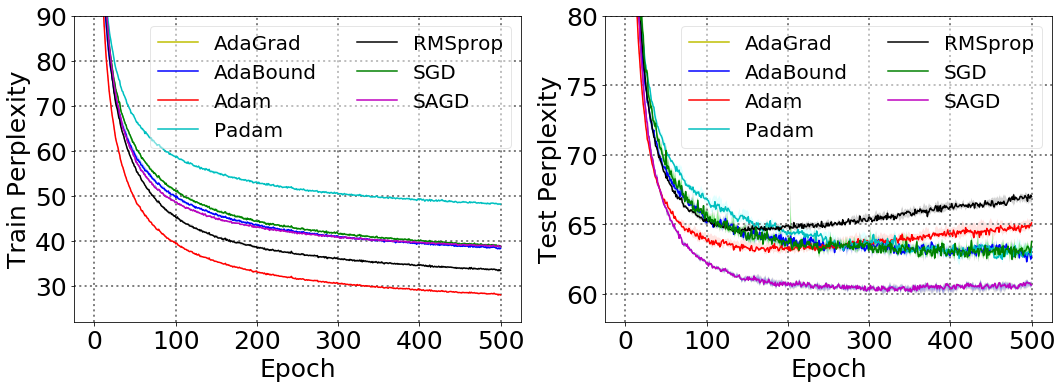
\includegraphics[width = 0.48 \textwidth ]{figure/new/3lstm2.png}
% }
%}
% \caption[]{Train and test perplexity of 2-layer LSTM and 3-layer LSTM. 
% Although adaptive methods such as AdGrad, Padam, Adam, and RMsprop achieves better training performance than \textsc{SAGD}, \textsc{SAGD} performs the best in terms of the test perplexity among all the methods.
%} 
% \label{fig:cifar10}
%\end{figure}


\vspace{0.05in}

\textbf{Recurrent Neural Network.}
An experiment on Penn Treebank is conducted for the language modeling task with 2-layer Long Short-Term Memory (LSTM)~\citep{Proc:Merity_ICLR18} network and 3-layer LSTM. We train them for a fixed budget of 500 epochs and omit the learning-rate decay. Perplexity is used as the metric to evaluate the performance and learning curves are plotted in Figure~\ref{fig:language}. 
For a 2-layer LSTM, we observe in Figure~\ref{fig:language} that RMSprop and Adam achieve a lower training perplexity than \textsc{SAGD}. 
However, \textsc{SAGD} performs the best in terms of the test perplexity. Specifically, \textsc{SAGD} achieves $60.66 \pm 0.05$ test perplexity. 
In particular, we observe that after 200 epochs, the test perplexity of RMSprop and Adam starts increasing, but the training perplexity continues decreasing (over-fitting occurs).  
For the 3-layer LSTM, Figure~\ref{fig:language} shows that the perplexity of Adam and RMSprop start increasing significantly after 150 epochs (\emph{over-fitting}) while the perplexity of \textsc{SAGD} keeps decreasing. \textsc{SAGD}, SGD and AdaBound perform better than Adam, and RMSprop in terms of over-fitting.
Table~\ref{tab:ppl} shows the best test perplexity of 2-layer LSTM and 3-layer LSTM for all the algorithms. We can observe that the \textsc{SAGD} achieves the best test perplexity $59.43 \pm 0.24$ among all the algorithms. 

\begin{table}[H]
\caption{ Test Perplexity of LSTMs on Penn Treebank. Bold number indicates the best result.}\label{tab:ppl}
	\resizebox{\columnwidth}{!}{%
\begin{tabular}{llllllll}
\toprule[1pt]
 & RMSprop      & Adam     & AdaBound    & SGD          & \textsc{SAGD}         \\ \hline
2-layer LSTM & 62.87 $\pm$ 0.05 & 66.02 $\pm$ 0.05  & 65.82 $\pm$0.08 & 65.96 $\pm$ 0.23 & \textbf{60.66 $\pm$ 0.05} \\
3-layer LSTM & 63.97 $\pm$ 018  & 63.23 $\pm$ 004   & 62.33 $\pm$0.07 & 62.51 $\pm$0.11  & \textbf{59.43 $\pm$ 0.24} \\
\toprule[1pt]
\end{tabular}
}\vspace{-0.05in}
\end{table}

% \begin{table}[H]
% \caption{ Test Perplexity of LSTMs on Penn Treebank. Bold number indicates the best result.}\label{tab:ppl}
% 	\resizebox{\columnwidth}{!}{%
% \begin{tabular}{llllllll}
% \toprule[1pt]
%  & RMSprop      & Adam         & AdaGrad      & Padam        & AdaBound    & SGD          & \textsc{SAGD}         \\ \hline
% 2-layer LSTM & 62.87 $\pm$ 0.05 & 60.58 $\pm$ 0.37 & 62.20 $\pm$ 0.29 & 62.85 $\pm$ 0.16 & 65.82 $\pm$0.08 & 65.96 $\pm$ 0.23 & \textbf{60.66 $\pm$ 0.05} \\
% 3-layer LSTM & 63.97 $\pm$ 018  & 63.23 $\pm$ 004  & 66.25 $\pm$ 0.31 & 66.45 $\pm$ 0.28 & 62.33 $\pm$0.07 & 62.51 $\pm$0.11  & \textbf{59.43 $\pm$ 0.24} \\
% \toprule[1pt]
% \end{tabular}
% }\vspace{-0.05in}
% \end{table}


\textbf{Bidirectional LSTM.}
We use a bi-directional LSTM architecture, as the concatenation of a forward LSTM and a backward LSTM as described in~\citep{Proc:Conneau_EMNLP17}.
We use $300$ dimensions as fixed word embeddings and set the learning rate following the method described above.
In Figure~\ref{fig:language}, we compare mini-batch SAGD to the following baselines: Adam~\citep{Proc:Kingma_ICLR15},  RMSprop~\citep{tige12}, and Adabound~\citep{Proc:Luo_ICLR19}. 
As in the language modeling task on PTB, we observe that whilst \textsc{SAGD} displays a worse loss perplexity than baseline methods, it keeps a low testing perplexity through the epochs.
This phenomena has been observed in all of our experiments and highlights the advantage of our proposed method to present \emph{reused} samples to the model as if they were fresh ones. 
Thus, over-fitting is less likely to happen and testing loss will remain low.
For instance, Adam achieves the best training perplexity, yet displays an increasing testing perplexity after a few epochs, which leads to low test accuracy.



\section{Conclusion}\label{sec: conclusion}

In this paper, we focus on the generalization ability of adaptive gradient methods. 
Concerned with the observation that adaptive gradient methods generalize worse than SGD for over-parameterized neural networks and given the limited theoretical understanding of the generalization of those methods,
we propose \textbf{S}table \textbf{A}daptive \textbf{G}radient \textbf{D}escent (\textsc{SAGD}) methods, which boost the generalization performance in both theory and practice through a novel use of differential privacy. 
The proposed algorithms generalize well with provable high-probability convergence bounds of the population gradient. 
Experimental studies highlight that the proposed algorithms are competitive and often better than baseline algorithms for training deep neural networks and demonstrate the aptitude of our method to avoid over-fitting through a differential privacy mechanism.

\clearpage

\section{Broader Impact}
We believe that our work stands in the line of several papers towards improving generalization and avoiding over-fitting.
Indeed, the basic principle of our method is to fit any given model, in particular deep model, using an intermediate differentially-private mechanisms allowing the model to fit fresh samples while passing over the same batch of $n$ observations.
The impact of such work is straightforward and could avoid learning, and thus reproducing at testing phase, the bias existent in the training dataset.



\bibliographystyle{plain}
\bibliography{standard}

\clearpage


\appendix
%%\section{Hyperparameter tunning}
%\input{app_setup.tex}

\section{Differential Privacy and Generalization Analysis} \label{sec: pri} \label{sec: pri}



\begin{comment}
\textbf{Assumptions}
\begin{enumerate}
    \item  $ f: \mathbb{R}^d \rightarrow \mathbb{R}$ is differentiable (not necessarily convex), bounded from below by $f^\star$,
and has L-Lipschitz gradient, i.e.,
\begin{equation}
    \nabla f(\w) -\nabla f(\w^\prime) \leq L \|\w-\w^\prime \|, ~ \forall \w, \w^\prime \in \cW
\end{equation}
\item  The noisy gradient is bounded:
\begin{equation}
    \|\tilde \g_t\|_2^2 \leq G
\end{equation}

\item  The $l_1$ norm of the individual gradient is bounded:
\begin{equation}
    \|\nabla \ell (\w,\z) \|_1 \leq G_1, \ \ \  \forall \w \in \cW, \z \in \cZ
\end{equation}
\end{enumerate}


\textbf{Generalization guarantee of differential privacy}




\begin{lemm} \label{lem: gen_basic}
Let $\cA$ be an $\epsilon$-differentially private gradient descent algorithm 
which has access to the training set $S$ of size $n$. Let $\w_t = \cA(S)$ be the parameters generated at each iteration $t \in [T]$ and $\hat \g_t$ be the empircal gradient on $S$. Them, for any $\sigma >0$, $\beta \geq 6\exp(\frac{-\sigma^2 n}{4G_1^2})$, if the privacy cost of $\cA$ satisfies $\epsilon \leq \frac{\sigma}{2G_1}$, we have
\begin{equation}
    \mathbb{P}\left\{ |\hat \g_t^i - \g_t^i| \geq  \sigma \right\} \leq \beta,
\end{equation}
for every $ i\in [d]$ and every $t \in [T]$.
\end{lemm}
\end{comment}



\begin{comment}
\begin{lemm} 
Let $\cA$ be an $(\epsilon, \delta)$-differentially private gradient descent algorithm 
which has access to the training set $S$ of size $n$. Let $\w_t = \cA(S)$ be the parameters generated at each iteration $t \in [T]$ and $\hat \g_t$ be the empircal gradient on $S$. Them, for any $\sigma >0$, $\beta > 0$, if the privacy cost of $\cA$ satisfies $\varepsilon \leq \frac{\sigma}{13}$, $\delta \leq \frac{\sigma \beta}{26 \ln(26/\sigma)}$ and the sample size $n \geq \frac{2\ln(8/\delta)}{\varepsilon^2}$, we have
\begin{equation}
    \mathbb{P}\left\{ |\hat \g_t^i - \g_t^i| \geq  \sigma \right\} \leq \beta,
\end{equation}
for every $ i\in [d]$ and every $t \in [T]$.
\end{lemm}
\end{comment}


%\textbf{Proof of Lemma \ref{lem: gen_adv}:} 



%Note that Lemma \ref{lem: gen_adv} is the instantiation of Corollary 8 from \cite{dwfe15}.


%\subsection{Proof of Lemma \ref{lemma dpp}:} 

%\begin{proof}
%At each iteration $t$, the algorithm is composed of two sequential parts: \textbf{DPG} to access the training set $S$ and compute $\tilde \g_t$, and parameter update based on estimated $\tilde \g_t$. We mark the \textbf{DPG} as part $\mathcal{A}$ and the gradient descent as part $\mathcal{B}$. We first show $\mathcal{A}$ preserves $\frac{G_1}{n\sigma}$-differential privacy. Then according to the \emph{post-processing property} of differential privacy (Proposition 2.1 in \cite{dwro2014}) we have $\mathcal{B} \circ \mathcal{A}$ is also $\frac{G_1}{n\sigma}$-differentially private.
	
%The part $\mathcal{A}$ (DPG-Lap) uses the basic tool from differential privacy, the ``Laplace Mechanism'' (Definition 3.3 in \citep{dwro2014}). 
%The Laplace Mechanism adds i.i.d. Laplace noise to each coordinate of the output. Adding noise from $Lap(\sigma)$ to a query of $G_1/n$
% sensitivity preserves $G_1/n\sigma$-differential privacy by ( Theorem 3.6 in \cite{dwro2014}).
 %Over $T$ iterations, we have $T$ applications of a DPG-Lap. By the advanced composition theorem (Theorem 3.20 in \cite{dwro2014}), $T$ applications of a $\frac{G_1}{n\sigma}$-differentially private algorithm is $(\frac{\sqrt{T \ln(1/\delta)} G_1}{n\sigma}, \delta)$-deferentially private. 
 %So SAGD with DPG-Lap is $(\frac{\sqrt{T \ln(2/\delta)} 2G_1}{n\sigma}, \delta)$-deferentially private.
%\end{proof}




%\subsection{Batch Sparse Vector Mechanism}

%\subsection{Proof of Lemma \ref{lemma: dpp-sparse}:}


By applying Theorem 8 from \citet{dwfe2015a} to gradient computation, we can get the Lemma \ref{lem: gen_adv}.

\lemgenadv*

\proof 
Theorem 8 in \citet{dwfe2015a}  shows that in order to achieve generalization error $\tau$ with probability $1-\rho$ for a $(\epsilon, \delta)$-differentially private algorithm (i.e., in order
to guarantee for every function $\phi_t$, $\forall t \in [T]$, we have $\mathbb{P}\left[\left|\mathcal{P}\left[\phi_t\right]-\mathcal{E}_{S}\left[\phi_t\right]\right| \geq \tau\right] \leq \rho$), where $\mathcal{P}\left[\phi_t\right]$ is the population value, $\mathcal{E}_{S}\left[\phi_t\right]$ is the empirical value evaluated on $S$ and $\rho$ and $\tau$ are any positive constant, we can set the $\epsilon \leq \frac{\tau}{13}$ and $\delta \leq \frac{\tau \rho}{26 \ln (26 / \tau)}$. In our context, $\tau = \sigma$, $\beta =\rho$, $\phi_t$ is 
the gradient computation function $\nabla \ell(\w_t,\z)$,  $\mathcal{P}\left[\phi_t\right]$ represents the population gradient $\g_t^i$, $\forall i\in [p]$, and $\mathcal{E}_{S}\left[\phi_t\right]$ represents the sample gradient $\hat \g_t^i$, $\forall i\in [p]$. Thus we have $\mathbb{P}\left\{\left|\hat{\mathbf{g}}_{t}^{i}-\mathbf{g}_{t}^{i}\right| \geq \tau\right\} \leq \rho$ if $\epsilon \leq \frac{\sigma}{13}, \delta \leq \frac{\sigma \beta}{26 \ln (26 / \sigma)}$.

\subsection{Proof of Lemma \ref{lemma dpp}}


\lemdpp*

\begin{proof}
At each iteration $t$, the algorithm is composed of two sequential parts: DPG to access the training set $S$ and compute $\tilde \g_t$, and parameter update based on estimated $\tilde \g_t$. We mark the DPG as part $\mathcal{A}$ and the gradient descent as part $\mathcal{B}$. We first show $\mathcal{A}$ preserves $\frac{G_1}{n\sigma}$-differential privacy. Then according to the \emph{post-processing property} of differential privacy (Proposition 2.1 in~\cite{dwro2014}) we have $\mathcal{B} \circ \mathcal{A}$ is also $\frac{G_1}{n\sigma}$-differentially private.
	
The part $\mathcal{A}$ (DPG-Lap) uses the basic tool from differential privacy, the ``Laplace Mechanism'' (Definition 3.3 in~\citep{dwro2014}). 
The Laplace Mechanism adds i.i.d. Laplace noise to each coordinate of the output. Adding noise from $Lap(\sigma)$ to a query of $G_1/n$
 sensitivity preserves $G_1/n\sigma$-differential privacy by ( Theorem 3.6 in~\cite{dwro2014}).
 Over $T$ iterations, we have $T$ applications of a DPG-Lap. By the advanced composition theorem (Theorem 3.20 in~\cite{dwro2014}), $T$ applications of a $\frac{G_1}{n\sigma}$-differentially private algorithm is $(\frac{\sqrt{T \ln(1/\delta)} G_1}{n\sigma}, \delta)$-differentially private. 
 So SAGD with DPG-Lap is $(\frac{\sqrt{T \ln(1/\delta)} 2G_1}{n\sigma}, \delta)$-differentially private.
\end{proof}

\subsection{Proof of Theorem \ref{thm: acc_basic}}

\theoaccbasic*

\begin{proof}
The concentration bound is decomposed into two parts:
\begin{equation}
    \begin{split}
    &\mathbb{P} 
    \left\{ \|\tilde \g_t - \g_t\| \geq \sqrt{d}\sigma(1+\mu)\right\} \\
    \leq&   
    \underbrace{ \mathbb{P}\left\{ \|\tilde \g_t - \hat \g_t\| \geq  \sqrt{d}\sigma \mu\right\} }_{\text{$T_1$: empirical error}} 
     + \underbrace{\mathbb{P}\left\{ \|\hat \g_t - \g_t\| \geq \sqrt{d}\sigma \right\}}_{\text{$T_2$: generalization error}} \nr
    \end{split}
\end{equation}
In the above inequality, there are two types of error we need to control. The first type of error, referred to as empirical error $T_1$, is the deviation between the differentially
private estimated gradient $\tilde \g_t$ and the empirical gradient $\hat \g_t$. The second type of error, referred to as generalization error $T_2$, is the deviation
between the empirical gradient $\hat \g_t$ and the population gradient $\g_t$. 

The second term $T_2$ can be bounded thorough the generalization guarantee of differential privacy. Recall that from  Lemma~\ref{lem: gen_adv}, under the condition in Theorem~\ref{thm: acc_sparse}, we have for all $t \in [T]$, $i \in [d]$: 
\begin{equation}
    \mathbb{P}\left\{ |\hat \g_t^i - \g_t^i| \geq  \sigma \right\} \leq \beta \nr
\end{equation}
So that we have 
\begin{equation}\label{eq: gen1}
\mathbb{P}\left\{ \|\hat \g_t - \g_t\| \geq  \sqrt{d}\sigma \right\} \leq \mathbb{P}\left\{ \|\hat \g_t - \g_t\|_\infty \geq  \sigma  \right\} \leq d \mathbb{P}\left\{ |\hat \g_t^i - \g_t^i| \geq  \sigma \right\} \leq d\beta 
\end{equation}

Now we bound the second term $T_1$. Recall that $\tilde \g_t = \hat \g_t + \b_t$, where $\b_t$ is a noise vector with each coordinate drawn from Laplace noise Lap$(\sigma)$. In this case, we have
\begin{align} \label{eq: acc1}
\mathbb{P}\left\{ \|\tilde \g_t - \hat \g_t\| \geq  \sqrt{d}\sigma \mu \right\}  \leq \mathbb{P} \left\{ \|\b_t\| \geq  \sqrt{d}\sigma \mu \right\}  &\leq \mathbb{P} \left\{ \|\b_t\|_\infty \geq  \sigma \mu \right\} \\ 
  &\leq d \mathbb{P} \left\{ |\b_t^i| \geq \sigma \mu \right\}\\
    &= d \exp(-\mu)
\end{align}

The second inequality comes from $\|\b_t\| \leq \sqrt{d}\|\b_t\|_\infty$. The
last equality comes from the property of Laplace distribution. Combine \eqref{eq: gen1} and \eqref{eq: acc1}, we complete the proof.
\end{proof}

\subsection{Proof of Lemma \ref{lemma: dpp-sparse}}

\lemdppsparse*

\begin{proof}
At each iteration $t$, the algorithm is composed of two sequential parts: DPG-Sparse (part $\mathcal{A}$) and parameter update based on estimated $\tilde \g_t$ (part $\mathcal{B}$).
%which accesses the training set $S$ and compute $\tilde \g_t$, and parameter update based on estimated $\tilde \g_t$. We mark the DPG-Sparse as part $\mathcal{A}$ and the gradient descent as part $\mathcal{B}$.
We first show $\mathcal{A}$ preserves $\frac{2G_1}{n\sigma}$-differential privacy. Then according to the \emph{post-processing property} of differential privacy (Proposition 2.1 in~\cite{dwro2014}) we have $\mathcal{B} \circ \mathcal{A}$ is also $\frac{2G_1}{n\sigma}$-differentially private.
	
The part $\mathcal{A}$ (DPG-Sparse) is a composition of basic tools from differential privacy, the ``Sparse Vector Algorithm'' (Algorithm 2 in~\citep{dwro2014}) and the ``Laplace Mechanism'' (Definition 3.3 in~\citep{dwro2014}). In our setting, the sparse vector algorithm takes as input a sequence of $T$ sensitivity $G_1/n$ queries, and for each query, attempts to determine whether the value of the query, evaluated on the private dataset $S_1$, is above a fixed threshold $\gamma + \tau$ or below it. In our instantiation, the  $S_1$ is the private data set, and each function corresponds to the gradient computation function $ \hat \g_t$ which is of sensitivity $G_1/n$. 
%SAGD is equivalent to the following procedure: we run the sparse vector algorithm for with $T$ queries corresponding to  gradient computation function $ \hat \g_t, t \in [T]$, and noise rate $\sigma$. 
By the privacy guarantee of the sparse vector algorithm, the sparse vector portion of SAGD satisfies $G_1/n\sigma$-differential privacy. The Laplace mechanism portion of SAGD
satisfies $G_1/n\sigma$-differential privacy by ( Theorem 3.6 in~\cite{dwro2014}). Finally, the composition of two mechanisms satisfies $\frac{2G_1}{n\sigma}$-differential privacy. For the sparse vector technique, only the query that fails the validation, corresponding to the `above threshold', release the privacy
of private dataset $S_1$ and pays a $\frac{2G_1}{n\sigma}$ privacy cost. 
Over all the iterations $T$, We have $C_{s}$ queries fail the validation.
Thus, by the advanced composition theorem (Theorem 3.20 in~\cite{dwro2014}), $C_{s}$ applications of a $\frac{2G}{n\sigma}$-differentially private algorithm is  $(\frac{\sqrt{C_{s} \ln(2/\delta)} 2G_1}{n\sigma}, \delta)$-differentially private. So SAGD with DPG-Sparse is $(\frac{\sqrt{C_{s} \ln(2/\delta)} 2G_1}{n\sigma}, \delta)$-differentially private.
\end{proof}
    


\subsection{Proof of Theorem \ref{thm: acc_sparse}:}

\theoaccsparse*

\begin{proof}
The concentration bound can be decomposed into two parts:
\begin{align}\notag
\mathbb{P}\left\{ \|\tilde \g_t - \g_t\| \geq \sqrt{d}\sigma(1+\mu)\right\}  \leq \underbrace{ \mathbb{P}\left\{ \|\tilde \g_t - \hat \g_{s_1,t}\| \geq \sqrt{d}\sigma \mu\right\} }_{\text{$T_1$: empirical error}} +  \underbrace{\mathbb{P}\left\{ \|\hat \g_{s_1,t} - \g_t\| \geq \sqrt{d}\sigma \right\}}_{\text{$T_2$: generalization error}}
\end{align}
%In the above inequality, there are two types of error we need to control. The first type of error, referred to as empirical error $T_1$, is the the deviation between the differentially
%private estimate gradient $\tilde \g_t$ and the empirical gradient $\hat \g_t$. The second type of error, referred to as generalization error $T_2$, is the deviation
%between the empirical gradient $\hat \g_t$ and the population gradient $\g_t$. 

%The second term $T_2$ can be bounded thorough the generalization guarantee of differential privacy. Recall that from  Lemma \ref{lem: gen_adv}, under the condition in Theorem \ref{thm: acc_sparse}, we have for all $t \in [T]$ and for all $i \in [d]$: 
%\begin{equation}
%    \mathbb{P}\left\{ |\hat \g_{s_1,t}^i - \g_t^i| \geq  \sigma \right\} \leq \beta
%\end{equation}
So that we have 
\begin{align} \notag
    \mathbb{P}\left\{ \|\hat \g_{s_1,t} - \g_t\| \geq  \sqrt{d}\sigma \right\} 
    &\leq \mathbb{P}\left\{ \|\hat \g_{s_1,t} - \g_t\|_\infty \geq  \sigma \right\} \\\notag
    &\leq d \mathbb{P}\left\{ |\hat \g_{s_1,t}^i - \g_t^i| \geq  \sigma \right\} \\\label{eq: gen2}
    &\leq d\beta 
\end{align}

Now we bound the second term $T_1$ by considering two cases, by depending on whether DPG-3 answers the query $\tilde \g_t$ by 
returning $\tilde \g_t = \hat \g_{s_1,t} + \v_t$ or by returning $\tilde \g_t = \hat \g_{s_2,t}$. In the first case, we have 
\begin{equation}
    \|\tilde \g_t - \hat \g_{s_1,t}\| = \|\v_t\| \nr
\end{equation}
and
\begin{equation}
\begin{split}
    \mathbb{P}\left\{ \|\tilde \g_t - \hat \g_{s_1,t}\| \geq \sqrt{d}\sigma \mu  \right\}  = \mathbb{P} \left\{ \|\v_t\| \geq  \sqrt{d}\sigma \mu \right\} \leq d \exp(-\mu) \nr
\end{split}
\end{equation}
The last inequality comes from the $\|\v_t\| \leq \sqrt{d}\|\v_t\|_\infty$ and properties of the Laplace distribution. 

In the second case, we have 
\begin{equation}
    \|\tilde \g_t - \hat \g_{s_1,t} \| = \| \hat \g_{s_2,t} -\hat \g_{s_1,t} \| \leq |\gamma| + |\tau| \nr
\end{equation}
and 
\begin{equation}
\begin{split}
\mathbb{P} \left\{ \|\tilde \g_t - \hat \g_{s_1,t}\| \geq \sqrt{d}\sigma \mu  \right\} =& \mathbb{P} \left\{ |\gamma| + |\tau| 
 \geq   \sqrt{d}\sigma \mu \right\} \\ 
 \leq&
  \mathbb{P} \left\{ |\gamma|  \geq   \frac{2}{6}\sqrt{d}\sigma \mu \right\} +  \mathbb{P} \left\{ |\tau|  \geq   \frac{4}{6}\sqrt{d}\sigma \mu \right\} \\
 =& 2\exp(-\sqrt{d}\mu /6) \nr
\end{split}
\end{equation}

Combining these two cases, we have
\begin{align}\notag 
\mathbb{P} 
\left\{ \|\tilde \g_t - \hat \g_{s_1,t}\| \geq \sqrt{d}\sigma \mu  \right\}  \leq & \max \left\{ 
\mathbb{P} \left\{ \|\v_t\| \geq  \sqrt{d}\sigma \mu \right\}, 
\mathbb{P} \left\{ |\gamma| + |\tau|
 \geq   \sqrt{d}\sigma \mu \right\}
\right\} \\\notag 
\leq& \max \left\{ d\exp(-\mu), 2\exp(-\sqrt{d}\mu /6) \right\} \\\label{eq: acc2}
=& d\exp(-\mu)
\end{align}

Combine \eqref{eq: gen2} and \eqref{eq: acc2}, we complete the proof.

\end{proof}


\clearpage
\section{Non-asymptotic Convergence analysis}
%\section{CONVERGENCE ANALYSIS}

In this section, we present the proof of Theorem \ref{thm: main_rmsprop}, \ref{thm: main_rmsprop_sparse}
\label{sec: thm2_proof}, \ref{thm: main_rmsprop_mini}.

\subsection{Proof of Theorem \ref{thm: main_rmsprop} and Theorem \ref{thm: main_rmsprop_sparse}}

The proof of Theorem \ref{thm: main_rmsprop} consists of two parts: We first prove that the convergence rate of a gradient-based iterative algorithm is related to the gradient concentration error $\alpha$ and its iteration 
time $T$. Then we combine the concentration error $\alpha$ achieved by SAGD with DPG-Lap in Theorem \ref{thm: acc_basic} with the first part to complete the proof of Theorem \ref{thm: main_rmsprop}. 
To simplify the analysis, we first use $\alpha$ and $\xi$ to denote the generalization error $\sqrt{d} \sigma(1+\mu)$ and probability $d \beta+d \exp (-\mu)$ in Theorem \ref{thm: acc_basic} in the following analysis. The details are presented in the following theorem.
\begin{theo} \label{thm: simp_gen}
Let $\tilde \g_1,...,\tilde \g_T$ be the noisy gradients generated in Algorithm 1 through DPG oracle over $T$ iterations.
Then, for every $t \in [T]$, $\tilde \g_t$ satisfies
%Let $\g_t = \nabla f(\w_t)$ be the population gradient at parameter $w_t$. For $t \in [T]$, the noisy gradient $\tilde \g_t$ from DPG with oracle satisfies
\begin{equation} \nr
    \mathbb{P}\{\|\tilde \g_t - \g_t\| \geq \alpha \} \leq \xi \, ,
\end{equation}
where the values of $\alpha$ and $\xi$ are given in Section \ref{sec: pri}. 
\end{theo}
With the guarantee of Theorem \ref{thm: simp_gen}, we have the following theorem showing the convergence of SAGD.
\begin{theo} \label{thm: opt_rmsprop}
 let $\eta_t = \eta$. Further more assume that $\nu$, $\beta$ and $\eta$ are chosen such that the following conditions satisfied: $\eta \leq \frac{\nu}{2L}$. 
 Under the Assumption A1 and A2, the Algorithm 1 with $T$ iterations, $\phi_t(\tilde \g_1,...,\tilde \g_t) = \tilde \g_t$ and $ \v_t = \left(1-\beta_{2}\right) \sum_{i=1}^{t} \beta_{2}^{t-i} \tilde \g_{i}^{2}$ achieves:
\begin{equation}\label{eq: opt_rmsprop}
 \min_{t = 1,..., T}\|\nabla f(x_t)\|^2 \leq
    \left(G+\nu \right) \times \left(   \frac{ f(\w_1) - f^\star}{\eta T} + \frac{3 \alpha^2}{4\nu}\right) \, ,
\end{equation}
with probability at least $1-T\xi$.
\end{theo}
We can now tackle the proof of our result stated in Theorem \ref{thm: opt_rmsprop}.
\begin{proof}
Using the update rule of RMSprop, we have $\phi_t(\tilde \g_1,...,\tilde \g_t) = \tilde \g_t$ and $ \psi_t(\tilde \g_1,...,\tilde \g_t) = \left(1-\beta_{2}\right) \sum_{i=1}^{t} \beta_{2}^{t-i} \tilde \g_{i}^{2}$.
Thus, we can rewrite the update of Algorithm \ref{algo: StAda} as:
\begin{equation}
\begin{split} \nr
    \w_{t+1} = \w_t - \eta_t \tilde  \g_t /(\sqrt{\v_t} + \nu) \ \ \text{and} \ \  \v_t = \left(1-\beta_{2}\right) \sum_{i=1}^{t} \beta_{2}^{t-i} \tilde \g_{i}^{2} \, .
\end{split}
\end{equation}
Let $\Delta_t = \tilde \g_t - g_t$, we obtain:
\begin{equation} \notag
\begin{split}
 & f (\w_{t+1}) \\
\leq & f(\w_t) + \left<\g_t, \w_{t+1}-\w_t\right> + \frac{L}{2} \left\|\w_{t+1}-\w_t \right\|^2\\ 
=& f(\w_t) -\eta_t \left<\g_t, \tilde \g_t/(\sqrt{\v_t} +\nu) \right> + \frac{L\eta_t^2}{2} \left\|\frac{\tilde \g_t}{(\sqrt{\v_t} +\nu)} \right\|^2\\ 
=& f(\w_t) -\eta_t \left<\g_t, \frac{\g_t +\Delta_t}{\sqrt{\v_t} +\nu} \right> + \frac{L\eta_t^2}{2}\left\|\frac{\g_t + \Delta_t}{\sqrt{\v_t} +\nu}\right\|^2 \\ 
\leq& f(\w_t) -\eta_t \left<\g_t, \frac{\g_t }{\sqrt{\v_t} +\nu}\right> -\eta_t \left<\g_t, \frac{\Delta_t }{\sqrt{\v_t} +\nu} \right> + L\eta_t^2\left(\left\|\frac{\g_t }{\sqrt{\v_t} +\nu}\right\|^2 + \left\|\frac{ \Delta_t}{\sqrt{\v_t} +\nu}\right\|^2   \right) \\ 
  =& f(\w_t) -\eta_t \sum_{i=1}^d \frac{\left[\g_t\right]_i^2}{\sqrt{\v_t^i} +\nu} - \eta_t \sum_{i=1}^d \frac{\g_t^i \Delta_t^i}{\sqrt{\v_t^i} +\nu} +  L\eta_t^2\left(\sum_{i=1}^d\frac{[\g_t]_i^2 }{(\sqrt{\v_t^i} +\nu)^2} + \sum_{i=1}^d\frac{[\Delta_t]_i^2 }{(\sqrt{\v_t^i} +\nu)^2} 
    \right) \\ 
 \leq& f(\w_t) -\eta_t \sum_{i=1}^d \frac{[\g_t]_i^2}{\sqrt{\v_t^i} +\nu}  + \frac{\eta_t}{2}\sum_{i=1}^d \frac{[\g_t]_i^2 + [\Delta_t]_i^2}{\sqrt{\v_t^i} +  +\nu}  + \frac{L\eta_t^2}{\nu}\left(\sum_{i=1}^d\frac{[\g_t]_i^2 }{\sqrt{\v_t^i} +\nu} + \sum_{i=1}^d\frac{[\Delta_t]_i^2 }{\sqrt{\v_t^i} +\nu}
    \right) \\ 
 = & f(\w_t) - \left(\eta_t -\frac{\eta_t}{2} - \frac{L\eta_t^2}{\nu} \right)\sum_{i=1}^d\frac{[\g_t]_i^2 }{\sqrt{\v_t^i} +\nu}  +\left(  \frac{\eta_t}{2} + \frac{L\eta_t^2}{\nu} \right)\sum_{i=1}^d\frac{[\Delta_t]_i^2 }{\sqrt{\v_t^i} +\nu}    \,.
 \end{split}
\end{equation}


Given the parameter setting from the theorem, we see the following condition hold:
\begin{equation} \nr
    \frac{L\eta_t}{\nu} \leq \frac{1}{4}.
\end{equation}
Then we obtain
\begin{align} 
\nr f(\w_{t+1})& \leq f(\w_t) - \frac{\eta}{4} \sum_{i=1}^{d} \frac{\left[\mathbf{g}_{t}\right]_{i}^{2}}{\sqrt{\mathbf{v}_{t}^{i}}+\nu}+\frac{3 \eta}{4} \sum_{i=1}^{d} \frac{\left[\Delta_{t}\right]_{i}^{2}}{\sqrt{\v_t^i} + \nu} \\ 
& \leq f(\w_t) - \frac{\eta}{G + \nu} \|\g_t\|^2 + \frac{3\eta}{4\epsilon} \|\Delta_t\|^2 \nr  \, .
\end{align}
The second inequality follows from the fact that $0 \leq \v_t^i \leq G^2$. Using the telescoping sum and rearranging the inequality,  we obtain
\begin{align} \nr
\frac{\eta}{G + \nu} \sum_{t=1}^T \|\g_t\|^2  \leq f(\w_1) - f^\star + \frac{3\eta}{4\epsilon} \sum_{t=1}^T  \|\Delta_t\|^2  \, .
\end{align}

Multiplying with $\frac{G +\nu}{\eta T}$ on both sides and with the guarantee in Theorem 1 that $\|\Delta_t\| \leq \alpha$ with probability at least $1-\xi$,  we obtain 
\begin{equation} \nr
\min_{t = 1,..., T}\|\g_t\|^2 \leq \left(G+\nu \right) \times \left(   \frac{ f(\w_1) - f^\star}{\eta T} + \frac{3 \alpha^2}{4\nu}\right)  \, ,
\end{equation}
with probability at least $1-T\xi$.\\


\end{proof}

\vspace{0.1in}

We may now present the proof of our Theorem \ref{thm: main_rmsprop}.
\theomainrmsprop*
\begin{proof}
First consider the gradient concentration bound achieved by SAGD (Theorem \ref{thm: acc_basic} and Theorem \ref{thm: acc_sparse}) that if $ \frac{2n\sigma^2}{G_1^2}\leq T \leq \frac{n^2 \sigma^4}{169 \ln(1/(\sigma \beta))G_1^2}$, we have 
\begin{equation}
\begin{split}
\mathbb{P}\left\{\|\tilde \g_t - \g_t\| \geq \sqrt{d}\sigma(1+\mu)\right\} \leq d\beta + d\exp(-\mu), \ \ \forall t \in [T].
\end{split} \nr
\end{equation}
Then bring the setting in Theorem \ref{thm: main_rmsprop} that $\sigma = 1/n^{1/3}$, let $\mu = \ln (1/\beta)$ and $\beta = 1/(d n^{5/3})$, we have
\begin{equation}
 \|\tilde \g_t - \g_t\|^2 \leq d(1+\ln d + \frac{5}{3}\ln n)^2/n^{2/3}    \nr  \, ,
\end{equation}
with probability at least $1- 1/n^{5/3}$, when we set $T = n^{2/3}/\left(169G_1^2(\ln d + \frac{7}{3}\ln n)\right)$. 

Connect this result with Theorem \ref{thm: opt_rmsprop}, so that we have $\alpha^2 = d(1+\ln d + \frac{5}{3}\ln n)^2/n^{2/3}$ and $\xi = 1/n^{5/3}$. Bring the value $\alpha^2$, $\xi$ and $T = n^{2/3}/\left(169G_1^2(\ln d + \frac{7}{3}\ln n)\right)$ into \eqref{eq: opt_rmsprop}, with $\rho_{n,d} = O \left(\ln n + \ln d \right)$, we have
\begin{align*}
\min_{t = 1,..., T}\|\nabla f(\w_t)\|^2 \leq O\left( \frac{\rho_{n,d} \left(f(\w_1) - f^\star \right)}{n^{2/3}} \right) + O \left( \frac{d \rho_{n,d}^2}{n^{2/3}}\right)\, ,
\end{align*}
with probability at least $1-O\left(\frac{1}{\rho_{n,d} n}\right)$ which concludes the proof.
\end{proof}


\theormspropsparse*


\begin{proof}
The proof of Theorem \ref{thm: main_rmsprop_sparse} follows the proof of Theorem \ref{thm: main_rmsprop} by considering the case $C_{s} = T$.
\end{proof}


\subsection{Proof of Theorem \ref{thm: main_rmsprop_mini}} 

\theomini*

\begin{proof} When mini-batch SAGD calls \textbf{DPG} to access each batch $s_k$ with size $m$ for $T$ times, we have mini-batch SAGD preserves $(\frac{\sqrt{T \ln(1/\delta)} G_1}{m\sigma}, \delta)$-deferential privacy for each batch $s_k$. Now consider the gradient concentration bound achieved by DPG-Lap (Theorem \ref{thm: acc_basic}) that if $ \frac{2m\sigma^2}{G_1^2}\leq T \leq \frac{m^2 \sigma^4}{169 \ln(1/(\sigma \beta))G_1^2}$, we have 
\begin{align*}
\mathbb{P}\left\{\|\tilde \g_t - \g_t\| \geq \sqrt{d}\sigma(1+\mu)\right\} \leq d\beta + d\exp(-\mu), \ \ \forall t \in [T]  \, .
\end{align*}
Then bring the setting in Theorem \ref{thm: main_rmsprop_mini} that $\sigma = 1/(nm)^{1/6}$, let $\mu = \ln (1/\beta)$ and $\beta = 1/(d n^{5/3})$, we have
\begin{equation}
 \|\tilde \g_t - \g_t\|^2 \leq d(1+\ln d + \frac{5}{3}\ln n)^2/n^{2/3}   \nr  \, ,
\end{equation}
with probability at least $1- 1/n^{5/3}$, when we set $T = (mn)^{1/3}/\left(169G_1^2(\ln d + \frac{7}{3}\ln n)\right)$. 


Connect this result with Theorem \ref{thm: opt_rmsprop}, so that we have $\alpha^2 = d(1+\ln d + \frac{5}{3}\ln n)^2/(mn)^{1/3}$ and $\xi = 1/n^{5/3}$. Bring the value $\alpha^2$, $\xi$ and $T = (mn)^{1/3}/\left(169G_1^2(\ln d + \frac{7}{3}\ln n)\right)$ into \eqref{eq: opt_rmsprop}, with $\rho_{n,d} = O \left(\ln n + \ln d \right)$, we have
\begin{align*}
\min_{t = 1,..., T}\|\nabla f(\w_t)\|^2 \leq O\left( \frac{\rho_{n,d} \left(f(\w_1) - f^\star \right)}{(mn)^{1/3}} \right) + O \left( \frac{d \rho_{n,d}^2}{(mn)^{1/3}}\right)  \, ,
\end{align*} 
with probability at least $1-O\left(\frac{1}{\rho_{n,d} n}\right)$. Here we complete the proof.

\end{proof}




%\section{Convergence Analysis of SAGD with the Update Rule of SGD, AdaGrad-Norm and AdaGrad}
%\input{app_opt_analysis.tex}

%\section{Main Theorems}
%\label{sec: main_thm}
%\input{app_main_thm.tex}

%-----------------------------------------------------------------------------
%\vspace{0.4cm}


%\section{Hyperparameter tunning}
%\input{app_setup.tex}

\section{Differential Privacy and Generalization Analysis} \label{sec: pri}





\begin{comment}
\textbf{Assumptions}
\begin{enumerate}
    \item  $ f: \mathbb{R}^d \rightarrow \mathbb{R}$ is differentiable (not necessarily convex), bounded from below by $f^\star$,
and has L-Lipschitz gradient, i.e.,
\begin{equation}
    \nabla f(\w) -\nabla f(\w^\prime) \leq L \|\w-\w^\prime \|, ~ \forall \w, \w^\prime \in \cW
\end{equation}
\item  The noisy gradient is bounded:
\begin{equation}
    \|\tilde \g_t\|_2^2 \leq G
\end{equation}

\item  The $l_1$ norm of the individual gradient is bounded:
\begin{equation}
    \|\nabla \ell (\w,\z) \|_1 \leq G_1, \ \ \  \forall \w \in \cW, \z \in \cZ
\end{equation}
\end{enumerate}


\textbf{Generalization guarantee of differential privacy}




\begin{lemm} \label{lem: gen_basic}
Let $\cA$ be an $\epsilon$-differentially private gradient descent algorithm 
which has access to the training set $S$ of size $n$. Let $\w_t = \cA(S)$ be the parameters generated at each iteration $t \in [T]$ and $\hat \g_t$ be the empircal gradient on $S$. Them, for any $\sigma >0$, $\beta \geq 6\exp(\frac{-\sigma^2 n}{4G_1^2})$, if the privacy cost of $\cA$ satisfies $\epsilon \leq \frac{\sigma}{2G_1}$, we have
\begin{equation}
    \mathbb{P}\left\{ |\hat \g_t^i - \g_t^i| \geq  \sigma \right\} \leq \beta,
\end{equation}
for every $ i\in [d]$ and every $t \in [T]$.
\end{lemm}
\end{comment}



\begin{comment}
\begin{lemm} 
Let $\cA$ be an $(\epsilon, \delta)$-differentially private gradient descent algorithm 
which has access to the training set $S$ of size $n$. Let $\w_t = \cA(S)$ be the parameters generated at each iteration $t \in [T]$ and $\hat \g_t$ be the empircal gradient on $S$. Them, for any $\sigma >0$, $\beta > 0$, if the privacy cost of $\cA$ satisfies $\varepsilon \leq \frac{\sigma}{13}$, $\delta \leq \frac{\sigma \beta}{26 \ln(26/\sigma)}$ and the sample size $n \geq \frac{2\ln(8/\delta)}{\varepsilon^2}$, we have
\begin{equation}
    \mathbb{P}\left\{ |\hat \g_t^i - \g_t^i| \geq  \sigma \right\} \leq \beta,
\end{equation}
for every $ i\in [d]$ and every $t \in [T]$.
\end{lemm}
\end{comment}

\subsection{Proof of Lemma~\ref{lem: gen_adv}}
By applying Theorem 8 from~\cite{Proc:Dwork_NIPS15} to gradient computation, we can get the Lemma~\ref{lem: gen_adv}.

\lemgenadv*

\proof 
Theorem 8 in~\cite{Proc:Dwork_NIPS15}  shows that in order to achieve generalization error $\tau$ with probability $1-\rho$ for an $(\epsilon, \delta)$-differentially private algorithm (i.e., in order
to guarantee for every function $\phi_t$, $\forall t \in [T]$, we have $\mathbb{P}\left[\left|\mathcal{P}\left[\phi_t\right]-\mathcal{E}_{S}\left[\phi_t\right]\right| \geq \tau\right] \leq \rho$), where $\mathcal{P}\left[\phi_t\right]$ is the population value, $\mathcal{E}_{S}\left[\phi_t\right]$ is the empirical value evaluated on $S$ and $\rho$ and $\tau$ are any positive constant, we can set the $\epsilon \leq \frac{\tau}{13}$ and $\delta \leq \frac{\tau \rho}{26 \ln (26 / \tau)}$. In our context, $\tau = \sigma$, $\beta =\rho$, $\phi_t$ is 
the gradient computation function $\nabla \ell(\w_t,\z)$,  $\mathcal{P}\left[\phi_t\right]$ represents the population gradient $\g_t^i/G$, $\forall i\in [p]$, and $\mathcal{E}_{S}\left[\phi_t\right]$ represents the sample gradient $\hat \g_t^i/G$, $\forall i\in [p]$. Thus we have $\mathbb{P}\left\{\left|\hat{\mathbf{g}}_{t}^{i}-\mathbf{g}_{t}^{i}\right|/G \geq \tau\right\} \leq \rho$ if $\epsilon \leq \frac{\sigma}{13}, \delta \leq \frac{\sigma \beta}{26 \ln (26 / \sigma)}$.

\subsection{Proof of Lemma~\ref{lemma dpp}}


\lemdpp*

\begin{proof}
At each iteration $t$, the algorithm is composed of two sequential parts: DPG to access the training set $S$ and compute $\tilde \g_t$, and parameter update based on estimated $\tilde \g_t$. We mark the DPG as part $\mathcal{A}$ and the gradient descent as part $\mathcal{B}$. We first show $\mathcal{A}$ preserves $\frac{G_1}{n\sigma}$-differential privacy. Then according to the \emph{post-processing property} of differential privacy (Proposition 2.1 in~\cite{Article:Dwork_2014}) we have $\mathcal{B} \circ \mathcal{A}$ is also $\frac{G_1}{n\sigma}$-differentially private.
	
The part $\mathcal{A}$ (DPG-Lap) uses the basic tool from differential privacy, the ``Laplace Mechanism'' (Definition 3.3 in~\citep{Article:Dwork_2014}). 
The Laplace Mechanism adds i.i.d. Laplace noise to each coordinate of the output. Adding noise from $Lap(\sigma)$ to a query of $G_1/n$
 sensitivity preserves $G_1/n\sigma$-differential privacy by ( Theorem 3.6 in~\cite{Article:Dwork_2014}).
 Over $T$ iterations, we have $T$ applications of a DPG-Lap. By the advanced composition theorem (Theorem 3.20 in~\cite{Article:Dwork_2014}), $T$ applications of a $\frac{G_1}{n\sigma}$-differentially private algorithm is $(\frac{\sqrt{T \ln(1/\delta)} G_1}{n\sigma}, \delta)$-differentially private. 
 So SAGD with DPG-Lap is $(\frac{\sqrt{T \ln(1/\delta)} 2G_1}{n\sigma}, \delta)$-differentially private.
\end{proof}

\subsection{Proof of Theorem~\ref{thm: acc_basic}}
\vspace{0.1in}

\theoaccbasic*

\begin{proof}
The concentration bound is decomposed into two parts:
\begin{equation}
    \begin{split}
\mathbb{P}  \left\{ \|\tilde \g_t - \g_t\| \geq \sqrt{d}\sigma(G+\mu)\right\} \leq
    \underbrace{ \mathbb{P}\left\{ \|\tilde \g_t - \hat \g_t\| \geq  \sqrt{d}\sigma \mu\right\} }_{\text{$T_1$: empirical error}} 
     + \underbrace{\mathbb{P}\left\{ \|\hat \g_t - \g_t\| \geq \sqrt{d}\sigma \right\}}_{\text{$T_2$: generalization error}} \nr \, .
    \end{split}
\end{equation}
In the above inequality, there are two types of error we need to control. The first type of error, referred to as empirical error $T_1$, is the deviation between the differentially
private estimated gradient $\tilde \g_t$ and the empirical gradient $\hat \g_t$. The second type of error, referred to as generalization error $T_2$, is the deviation
between the empirical gradient $\hat \g_t$ and the population gradient $\g_t$. 

The second term $T_2$ can be bounded thorough the generalization guarantee of differential privacy. Recall that from  Lemma~\ref{lem: gen_adv}, under the condition in Theorem~\ref{thm: acc_sparse}, we have for all $t \in [T]$, $i \in [d]$: 
\begin{equation}
    \mathbb{P}\left\{ |\hat \g_t^i - \g_t^i| \geq  G \sigma \right\} \leq \beta \nr \, .
\end{equation}
So that we have 
\begin{equation}\label{eq: gen1}
\mathbb{P}\left\{ \|\hat \g_t - \g_t\| \geq  \sqrt{d}G \sigma \right\} \leq \mathbb{P}\left\{ \|\hat \g_t - \g_t\|_\infty \geq  G \sigma  \right\} \leq d \mathbb{P}\left\{ |\hat \g_t^i - \g_t^i| \geq  G \sigma \right\} \leq d\beta \, .
\end{equation}

Now we bound the second term $T_1$. Recall that $\tilde \g_t = \hat \g_t + \b_t$, where $\b_t$ is a noise vector with each coordinate drawn from Laplace noise Lap$(\sigma)$. In this case, we have
\begin{align} \label{eq: acc1}
\mathbb{P}\left\{ \|\tilde \g_t - \hat \g_t\| \geq  \sqrt{d}\sigma \mu \right\}  \leq \mathbb{P} \left\{ \|\b_t\| \geq  \sqrt{d}\sigma \mu \right\}  &\leq \mathbb{P} \left\{ \|\b_t\|_\infty \geq  \sigma \mu \right\} 
  \leq d \mathbb{P} \left\{ |\b_t^i| \geq \sigma \mu \right\} = d \exp(-\mu) \, .
\end{align}
The second inequality comes from $\|\b_t\| \leq \sqrt{d}\|\b_t\|_\infty$. The
last equality comes from the property of Laplace distribution. Combine \eqref{eq: gen1} and \eqref{eq: acc1}, we complete the proof.
\end{proof}

\subsection{Proof of Lemma~\ref{lemma: dpp-sparse}}

\lemdppsparse*

\begin{proof}
At each iteration $t$, the algorithm is composed of two sequential parts: DPG-Sparse (part $\mathcal{A}$) and parameter update based on estimated $\tilde \g_t$ (part $\mathcal{B}$).
%which accesses the training set $S$ and compute $\tilde \g_t$, and parameter update based on estimated $\tilde \g_t$. We mark the DPG-Sparse as part $\mathcal{A}$ and the gradient descent as part $\mathcal{B}$.
We first show $\mathcal{A}$ preserves $\frac{2G_1}{n\sigma}$-differential privacy. Then according to the \emph{post-processing property} of differential privacy (Proposition 2.1 in~\cite{Article:Dwork_2014}) we have $\mathcal{B} \circ \mathcal{A}$ is also $\frac{2G_1}{n\sigma}$-differentially private.
	
The part $\mathcal{A}$ (DPG-Sparse) is a composition of basic tools from differential privacy, the ``Sparse Vector Algorithm'' (Algorithm 2 in~\citep{Article:Dwork_2014}) and the ``Laplace Mechanism'' (Definition 3.3 in~\citep{Article:Dwork_2014}). In our setting, the sparse vector algorithm takes as input a sequence of $T$ sensitivity $G_1/n$ queries, and for each query, attempts to determine whether the value of the query, evaluated on the private dataset $S_1$, is above a fixed threshold $\gamma + \tau$ or below it. In our instantiation, the  $S_1$ is the private data set, and each function corresponds to the gradient computation function $ \hat \g_t$ which is of sensitivity $G_1/n$. 
%SAGD is equivalent to the following procedure: we run the sparse vector algorithm for with $T$ queries corresponding to  gradient computation function $ \hat \g_t, t \in [T]$, and noise rate $\sigma$. 
By the privacy guarantee of the sparse vector algorithm, the sparse vector portion of SAGD satisfies $G_1/n\sigma$-differential privacy. The Laplace mechanism portion of SAGD
satisfies $G_1/n\sigma$-differential privacy by ( Theorem 3.6 in~\cite{Article:Dwork_2014}). Finally, the composition of two mechanisms satisfies $\frac{2G_1}{n\sigma}$-differential privacy. For the sparse vector technique, only the query that fails the validation, corresponding to the `above threshold', release the privacy
of private dataset $S_1$ and pays a $\frac{2G_1}{n\sigma}$ privacy cost. 
Over all the iterations $T$, We have $C_{s}$ queries fail the validation.
Thus, by the advanced composition theorem (Theorem 3.20 in~\cite{Article:Dwork_2014}), $C_{s}$ applications of a $\frac{2G}{n\sigma}$-differentially private algorithm is  $(\frac{\sqrt{C_{s} \ln(2/\delta)} 2G_1}{n\sigma}, \delta)$-differentially private. So SAGD with DPG-Sparse is $(\frac{\sqrt{C_{s} \ln(2/\delta)} 2G_1}{n\sigma}, \delta)$-differentially private.
\end{proof}
    


\subsection{Proof of Theorem~\ref{thm: acc_sparse}:}

\vspace{0.1in}

\theoaccsparse*

\begin{proof}
The concentration bound can be decomposed into two parts:
\begin{align}\notag
\mathbb{P}\left\{ \|\tilde \g_t - \g_t\| \geq \sqrt{d}\sigma(1+\mu)\right\}  \leq \underbrace{ \mathbb{P}\left\{ \|\tilde \g_t - \hat \g_{s_1,t}\| \geq \sqrt{d}\sigma \mu\right\} }_{\text{$T_1$: empirical error}} +  \underbrace{\mathbb{P}\left\{ \|\hat \g_{s_1,t} - \g_t\| \geq \sqrt{d}\sigma \right\}}_{\text{$T_2$: generalization error}} \, ,
\end{align}
%In the above inequality, there are two types of error we need to control. The first type of error, referred to as empirical error $T_1$, is the the deviation between the differentially
%private estimate gradient $\tilde \g_t$ and the empirical gradient $\hat \g_t$. The second type of error, referred to as generalization error $T_2$, is the deviation
%between the empirical gradient $\hat \g_t$ and the population gradient $\g_t$. 

%The second term $T_2$ can be bounded thorough the generalization guarantee of differential privacy. Recall that from  Lemma~\ref{lem: gen_adv}, under the condition in Theorem~\ref{thm: acc_sparse}, we have for all $t \in [T]$ and for all $i \in [d]$: 
%\begin{equation}
%    \mathbb{P}\left\{ |\hat \g_{s_1,t}^i - \g_t^i| \geq  \sigma \right\} \leq \beta
%\end{equation}
which yields
\begin{align} \label{eq: gen2}
    \mathbb{P}\left\{ \|\hat \g_{s_1,t} - \g_t\| \geq  \sqrt{d}\sigma \right\} \leq \mathbb{P}\left\{ \|\hat \g_{s_1,t} - \g_t\|_\infty \geq  \sigma \right\} \leq d \mathbb{P}\left\{ |\hat \g_{s_1,t}^i - \g_t^i| \geq  \sigma \right\} \leq d\beta  \, .
\end{align}

Now we bound the second term $T_1$ by considering two cases, by depending on whether DPG-3 answers the query $\tilde \g_t$ by 
returning $\tilde \g_t = \hat \g_{s_1,t} + \v_t$ or by returning $\tilde \g_t = \hat \g_{s_2,t}$. In the first case, we have 
\begin{equation}
    \|\tilde \g_t - \hat \g_{s_1,t}\| = \|\v_t\| \nr
\end{equation}
and
\begin{equation}
\begin{split}
    \mathbb{P}\left\{ \|\tilde \g_t - \hat \g_{s_1,t}\| \geq \sqrt{d}\sigma \mu  \right\}  = \mathbb{P} \left\{ \|\v_t\| \geq  \sqrt{d}\sigma \mu \right\} \leq d \exp(-\mu) \nr \, .
\end{split}
\end{equation}
The last inequality comes from the $\|\v_t\| \leq \sqrt{d}\|\v_t\|_\infty$ and properties of the Laplace distribution. 

In the second case, we have 
\begin{equation}
    \|\tilde \g_t - \hat \g_{s_1,t} \| = \| \hat \g_{s_2,t} -\hat \g_{s_1,t} \| \leq |\gamma| + |\tau| \nr
\end{equation}
and 
\begin{equation}
\begin{split}
\mathbb{P} \left\{ \|\tilde \g_t - \hat \g_{s_1,t}\| \geq \sqrt{d}\sigma \mu  \right\} =& \mathbb{P} \left\{ |\gamma| + |\tau| 
 \geq   \sqrt{d}\sigma \mu \right\} \\ 
 \leq&
  \mathbb{P} \left\{ |\gamma|  \geq   \frac{2}{6}\sqrt{d}\sigma \mu \right\} +  \mathbb{P} \left\{ |\tau|  \geq   \frac{4}{6}\sqrt{d}\sigma \mu \right\} \\
 =& 2\exp(-\sqrt{d}\mu /6) \nr \, .
\end{split}
\end{equation}

Combining these two cases, we have
\begin{align}\notag 
\mathbb{P} 
\left\{ \|\tilde \g_t - \hat \g_{s_1,t}\| \geq \sqrt{d}\sigma \mu  \right\}  \leq & \max \left\{ 
\mathbb{P} \left\{ \|\v_t\| \geq  \sqrt{d}\sigma \mu \right\}, 
\mathbb{P} \left\{ |\gamma| + |\tau|
 \geq   \sqrt{d}\sigma \mu \right\}
\right\} \\\notag 
\leq& \max \left\{ d\exp(-\mu), 2\exp(-\sqrt{d}\mu /6) \right\} \\\label{eq: acc2}
=& d\exp(-\mu) \, .
\end{align}

 We complete the proof by combining \eqref{eq: gen2} and \eqref{eq: acc2}.

\end{proof}



\vspace{0.2in}

\section{Non-asymptotic Convergence analysis}


In this section, we present the proofs for Theorems~\ref{thm: main_rmsprop},~\ref{thm: main_rmsprop_sparse}
\label{sec: thm2_proof},~\ref{thm: main_rmsprop_mini}.

\subsection{Proof of Theorem~\ref{thm: main_rmsprop} and Theorem~\ref{thm: main_rmsprop_sparse}}

The proof of Theorem~\ref{thm: main_rmsprop} consists of two parts: We first prove that the convergence rate of a gradient-based iterative algorithm is related to the gradient concentration error $\alpha$ and its iteration 
time $T$. Then we combine the concentration error $\alpha$ achieved by SAGD with DPG-Lap in Theorem~\ref{thm: acc_basic} with the first part to complete the proof of Theorem~\ref{thm: main_rmsprop}. 
To simplify the analysis, we first use $\alpha$ and $\xi$ to denote the generalization error $\sqrt{d} \sigma(G+\mu)$ and probability $d \beta+d \exp (-\mu)$ in Theorem~\ref{thm: acc_basic} in the following analysis. The details are presented in the following theorem.

\vspace{0.05in}

\begin{thm} \label{thm: simp_gen}
Let $\tilde \g_1,...,\tilde \g_T$ be the noisy gradients generated in Algorithm 1 through DPG oracle over $T$ iterations.
Then, for every $t \in [T]$, $\tilde \g_t$ satisfies
%Let $\g_t = \nabla f(\w_t)$ be the population gradient at parameter $w_t$. For $t \in [T]$, the noisy gradient $\tilde \g_t$ from DPG with oracle satisfies
\begin{equation} \nr
    \mathbb{P}\{\|\tilde \g_t - \g_t\| \geq \alpha \} \leq \xi \, ,
\end{equation}
where the values of $\alpha$ and $\xi$ are given in Section~\ref{sec: pri}. 
\end{thm}

%\vspace{0.2in}

With the guarantee of Theorem~\ref{thm: simp_gen}, we have the following theorem showing the convergence of SAGD.

\begin{thm} \label{thm: opt_rmsprop}
 Let $\eta_t = \eta$. Further more assume that $\nu$, $\beta$ and $\eta$ are chosen such that the following conditions satisfied: $\eta \leq \frac{\nu}{2L}$. 
 Under the Assumption A1 and A2, the Algorithm 1 with $T$ iterations, $\phi_t(\tilde \g_1,...,\tilde \g_t) = \tilde \g_t$ and $ \v_t = \left(1-\beta_{2}\right) \sum_{i=1}^{t} \beta_{2}^{t-i} \tilde \g_{i}^{2}$ achieves:
\begin{equation}\label{eq: opt_rmsprop}
 \min_{t = 1,..., T}\|\nabla f(x_t)\|^2 \leq
    \left(G+\nu \right) \times \left(   \frac{ f(\w_1) - f^\star}{\eta T} + \frac{3 \alpha^2}{4\nu}\right) \, ,
\end{equation}
with probability at least $1-T\xi$.
\end{thm}
We can now tackle the proof of our result stated in Theorem~\ref{thm: opt_rmsprop}.
\begin{proof}
Using the update rule of RMSprop, we have $\phi_t(\tilde \g_1,...,\tilde \g_t) = \tilde \g_t$ and $ \psi_t(\tilde \g_1,...,\tilde \g_t) = \left(1-\beta_{2}\right) \sum_{i=1}^{t} \beta_{2}^{t-i} \tilde \g_{i}^{2}$.
Thus, we can rewrite the update of Algorithm~\ref{algo: StAda} as:
\begin{equation}
\begin{split} \nr
    \w_{t+1} = \w_t - \eta_t \tilde  \g_t /(\sqrt{\v_t} + \nu) \ \ \text{and} \ \  \v_t = \left(1-\beta_{2}\right) \sum_{i=1}^{t} \beta_{2}^{t-i} \tilde \g_{i}^{2} \, .
\end{split}
\end{equation}
Let $\Delta_t = \tilde \g_t - g_t$, we obtain:
\begin{equation} \notag
\begin{split}
 & f (\w_{t+1}) \\
\leq & f(\w_t) + \left<\g_t, \w_{t+1}-\w_t\right> + \frac{L}{2} \left\|\w_{t+1}-\w_t \right\|^2\\ 
=& f(\w_t) -\eta_t \left<\g_t, \tilde \g_t/(\sqrt{\v_t} +\nu) \right> + \frac{L\eta_t^2}{2} \left\|\frac{\tilde \g_t}{(\sqrt{\v_t} +\nu)} \right\|^2\\ 
=& f(\w_t) -\eta_t \left<\g_t, \frac{\g_t +\Delta_t}{\sqrt{\v_t} +\nu} \right> + \frac{L\eta_t^2}{2}\left\|\frac{\g_t + \Delta_t}{\sqrt{\v_t} +\nu}\right\|^2 \\ 
\leq& f(\w_t) -\eta_t \left<\g_t, \frac{\g_t }{\sqrt{\v_t} +\nu}\right> -\eta_t \left<\g_t, \frac{\Delta_t }{\sqrt{\v_t} +\nu} \right> + L\eta_t^2\left(\left\|\frac{\g_t }{\sqrt{\v_t} +\nu}\right\|^2 + \left\|\frac{ \Delta_t}{\sqrt{\v_t} +\nu}\right\|^2   \right) \\ 
  =& f(\w_t) -\eta_t \sum_{i=1}^d \frac{\left[\g_t\right]_i^2}{\sqrt{\v_t^i} +\nu} - \eta_t \sum_{i=1}^d \frac{\g_t^i \Delta_t^i}{\sqrt{\v_t^i} +\nu} +  L\eta_t^2\left(\sum_{i=1}^d\frac{[\g_t]_i^2 }{(\sqrt{\v_t^i} +\nu)^2} + \sum_{i=1}^d\frac{[\Delta_t]_i^2 }{(\sqrt{\v_t^i} +\nu)^2} 
    \right) \\ 
 \leq& f(\w_t) -\eta_t \sum_{i=1}^d \frac{[\g_t]_i^2}{\sqrt{\v_t^i} +\nu}  + \frac{\eta_t}{2}\sum_{i=1}^d \frac{[\g_t]_i^2 + [\Delta_t]_i^2}{\sqrt{\v_t^i} +  +\nu}  + \frac{L\eta_t^2}{\nu}\left(\sum_{i=1}^d\frac{[\g_t]_i^2 }{\sqrt{\v_t^i} +\nu} + \sum_{i=1}^d\frac{[\Delta_t]_i^2 }{\sqrt{\v_t^i} +\nu}
    \right) \\ 
 = & f(\w_t) - \left(\eta_t -\frac{\eta_t}{2} - \frac{L\eta_t^2}{\nu} \right)\sum_{i=1}^d\frac{[\g_t]_i^2 }{\sqrt{\v_t^i} +\nu}  +\left(  \frac{\eta_t}{2} + \frac{L\eta_t^2}{\nu} \right)\sum_{i=1}^d\frac{[\Delta_t]_i^2 }{\sqrt{\v_t^i} +\nu}    \,.
 \end{split}
\end{equation}


Given the parameter setting from the theorem, we see the following condition hold:
\begin{equation} \nr
    \frac{L\eta_t}{\nu} \leq \frac{1}{4}.
\end{equation}
Then we obtain
\begin{align} 
\nr f(\w_{t+1})& \leq f(\w_t) - \frac{\eta}{4} \sum_{i=1}^{d} \frac{\left[\mathbf{g}_{t}\right]_{i}^{2}}{\sqrt{\mathbf{v}_{t}^{i}}+\nu}+\frac{3 \eta}{4} \sum_{i=1}^{d} \frac{\left[\Delta_{t}\right]_{i}^{2}}{\sqrt{\v_t^i} + \nu} \\ 
& \leq f(\w_t) - \frac{\eta}{G + \nu} \|\g_t\|^2 + \frac{3\eta}{4\epsilon} \|\Delta_t\|^2 \nr  \, .
\end{align}
The second inequality follows from the fact that $0 \leq \v_t^i \leq G^2$. Using the telescoping sum and rearranging the inequality,  we obtain
\begin{align} \nr
\frac{\eta}{G + \nu} \sum_{t=1}^T \|\g_t\|^2  \leq f(\w_1) - f^\star + \frac{3\eta}{4\epsilon} \sum_{t=1}^T  \|\Delta_t\|^2  \, .
\end{align}

Multiplying with $\frac{G +\nu}{\eta T}$ on both sides and with the guarantee in Theorem 1 that $\|\Delta_t\| \leq \alpha$ with probability at least $1-\xi$,  we obtain 
\begin{equation} \nr
\min_{t = 1,..., T}\|\g_t\|^2 \leq \left(G+\nu \right) \times \left(   \frac{ f(\w_1) - f^\star}{\eta T} + \frac{3 \alpha^2}{4\nu}\right)  \, ,
\end{equation}
with probability at least $1-T\xi$.\\


\end{proof}

\vspace{0.1in}

We now present the proof of our Theorem~\ref{thm: main_rmsprop}.
\theomainrmsprop*
\begin{proof}
First consider the gradient concentration bound achieved by SAGD (Theorem~\ref{thm: acc_basic} and Theorem~\ref{thm: acc_sparse}) that if $ \frac{2n\sigma^2}{G_1^2}\leq T \leq \frac{n^2 \sigma^4}{169 \ln(1/(\sigma \beta))G_1^2}$, we have 
\begin{equation}
\begin{split}
\mathbb{P}\left\{\|\tilde \g_t - \g_t\| \geq \sqrt{d}\sigma(G+\mu)\right\} \leq d\beta + d\exp(-\mu), \ \ \forall t \in [T].
\end{split} \nr
\end{equation}
Then bring the setting in Theorem~\ref{thm: main_rmsprop} that $\sigma = 1/n^{1/3}$, let $\mu = \ln (1/\beta)$ and $\beta = 1/(d n^{5/3})$, we have
\begin{equation}
 \|\tilde \g_t - \g_t\|^2 \leq d(1+\ln d + \frac{5}{3}\ln n)^2/n^{2/3}    \nr  \, ,
\end{equation}
with probability at least $1- 1/n^{5/3}$, when we set $T = n^{2/3}/\left(169G_1^2(\ln d + \frac{7}{3}\ln n)\right)$. 

Connect this result with Theorem~\ref{thm: opt_rmsprop}, so that we have $\alpha^2 = d(1+\ln d + \frac{5}{3}\ln n)^2/n^{2/3}$ and $\xi = 1/n^{5/3}$. Bring the value $\alpha^2$, $\xi$ and $T = n^{2/3}/\left(169G_1^2(\ln d + \frac{7}{3}\ln n)\right)$ into \eqref{eq: opt_rmsprop}, with $\rho_{n,d} = O \left(\ln n + \ln d \right)$, we have
\begin{align*}
\min_{t = 1,..., T}\|\nabla f(\w_t)\|^2 \leq O\left( \frac{\rho_{n,d} \left(f(\w_1) - f^\star \right)}{n^{2/3}} \right) + O \left( \frac{d \rho_{n,d}^2}{n^{2/3}}\right)\, ,
\end{align*}
with probability at least $1-O\left(\frac{1}{\rho_{n,d} n}\right)$ which concludes the proof.
\end{proof}


\theormspropsparse*


\begin{proof}
The proof of Theorem~\ref{thm: main_rmsprop_sparse} follows the proof of Theorem~\ref{thm: main_rmsprop} by considering the case $C_{s} = T$.
\end{proof}

\newpage

\subsection{Proof of Theorem~\ref{thm: main_rmsprop_mini}} 

\theomini*

\begin{proof} When mini-batch SAGD calls \textbf{DPG} to access each batch $s_k$ with size $m$ for $T$ times, we have mini-batch SAGD preserves $(\frac{\sqrt{T \ln(1/\delta)} G_1}{m\sigma}, \delta)$-deferential privacy for each batch $s_k$. Now consider the gradient concentration bound achieved by DPG-Lap (Theorem~\ref{thm: acc_basic}) that if $ \frac{2m\sigma^2}{G_1^2}\leq T \leq \frac{m^2 \sigma^4}{169 \ln(1/(\sigma \beta))G_1^2}$, we have 
\begin{align*}
\mathbb{P}\left\{\|\tilde \g_t - \g_t\| \geq \sqrt{d}\sigma(G +\mu)\right\} \leq d\beta + d\exp(-\mu), \ \ \forall t \in [T]  \, .
\end{align*}
Then bring the setting in Theorem~\ref{thm: main_rmsprop_mini} that $\sigma = 1/(nm)^{1/6}$, let $\mu = \ln (1/\beta)$ and $\beta = 1/(d n^{5/3})$, we have
\begin{equation}
 \|\tilde \g_t - \g_t\|^2 \leq d(1+\ln d + \frac{5}{3}\ln n)^2/n^{2/3}   \nr  \, ,
\end{equation}
with probability at least $1- 1/n^{5/3}$, when we set epoch $T = m^{4 / 3} /\left(n^{2 / 3} 169 G_{1}^{2}\left(\ln d+\frac{7}{3} \ln n\right)\right)$. 


Connect this result with Theorem~\ref{thm: opt_rmsprop}, so that we have $\alpha^2 = d(1+\ln d + \frac{5}{3}\ln n)^2/(mn)^{1/3}$ and $\xi = 1/n^{5/3}$. Bring the value $\alpha^2$, $\xi$ and total iteration number to be $T \times n/m$ with $T = (mn)^{1/3}/\left(169G_1^2(\ln d + \frac{7}{3}\ln n)\right)$ into \eqref{eq: opt_rmsprop}, with $\rho_{n,d} = O \left(\ln n + \ln d \right)$, we have
\begin{align*}
\min_{t = 1,..., T}\|\nabla f(\w_t)\|^2 \leq O\left( \frac{\rho_{n,d} \left(f(\w_1) - f^\star \right)}{(mn)^{1/3}} \right) + O \left( \frac{d \rho_{n,d}^2}{(mn)^{1/3}}\right)  \, ,
\end{align*} 
with probability at least $1-O\left(\frac{1}{\rho_{n,d} n}\right)$. Here we complete the proof.

\end{proof}


\end{document} 
